% !TeX root = ../main.tex

\chapter{基于强化学习的LLM Agent服务系统全局调度算法}\label{chap:agent-routing}
%第\ref{chap:adasched}章探讨了深度学习训练集群的弹性资源分配问题，主要面向生命周期较长、资源需求相对静态的训练作业，
%利用强化学习优化了训练性能与截止时间满足率。然而，在线大语言模型推理，尤其是基于智能体（Agent）的多轮工作流，
%在负载特征与优化目标上与训练作业存在本质差异。Agent推理请求生命周期短、负载动态性强，且工作流通常呈现为多节点构成的有向图结构，
%引入了复杂的请求间依赖，传统的训练调度范式已难以适用。

随着大模型能力的不断提升，LLM Agent正逐步成为新一代AI应用范式。
在多租户推理服务集群中，如何将Agent产生的多轮交互与工具调用请求高效地路由至底层多个LLM实例，
已成为决定其端到端延迟与集群资源利用率的核心瓶颈。
%因此，本章将研究视角转向LLM Agent服务集群的全局调度问题。

为此，本章提出并设计了一种面向LLM Agent服务系统的全局调度算法 RAGS。
该方法结合了感知Agent工作流的排队策略 DynA 与基于强化学习的全局分发算法，
旨在显著降低工作流的端到端延迟。
本章首先分析了LLM Agent服务系统的现状与全局路由面临的核心挑战，
接着详细介绍了面向Agent工作流的排队算法设计与基于强化学习的分发算法设计，
最后通过实验全面评估所提方法的有效性。

%\section{LLM Agent服务系统概述}\label{sec:agent-overview}
\section{问题描述}\label{subsec:routing-challenges}

如本文第\ref{sec:llm-sched-survey}节所述，
LLM推理服务系统通常采用分层调度架构（如图~\ref{fig:agent-system-arch} 所示）。
其中全局调度器承担两项核心决策任务：
一是决定请求的执行顺序（排队策略），二是确定请求的目标实例（分发策略）。
基于该架构与Agent工作流的基础概念，本节将进一步挖掘Agent工作流的深层特征，
旨在为后续全局调度器的排队策略与分发策略的设计奠定基础。

\subsection{LLM Agent的工作流特征}\label{subsec:agent-workflow}

为全面了解LLM Agent的特征，本文对 GitHub 等开源社区中的主流 Agent 
项目~\cite{aws2026genaichatbot,cognitivetech2026ollama,opencode2026terminal} 
展开调研，并系统分析了聊天机器人、代码生成、文档摘要等典型工作流范式。
如图~\ref{fig:agent-dag} 所示，典型的 Agent 工作流可抽象为一种有向图结构：
图中的每个节点表征单次 LLM 推理请求或外部工具调用，而边则严格刻画了节点间的数据流向与逻辑依赖。
基于该有向图拓扑，Agent 请求在系统层面主要呈现出以下显著特征：

\begin{figure}[htbp]
  \centering
  % --- 第一排：子图 (a) 和 (b) ---
  \begin{subfigure}[b]{0.48\textwidth}
    \centering
    \includegraphics[width=\textwidth]{figures/4.5.a.png}
    \caption{聊天机器人Agent工作流}
    \label{fig:agent-dag-a}
  \end{subfigure}
  \hfill % 使用 hfill 将两个子图推向两边，中间留出空白对齐
  \begin{subfigure}[b]{0.48\textwidth}
    \centering
    \includegraphics[width=\textwidth]{figures/4.5.b.png}
    \caption{MapReduce文档总结Agent工作流}
    \label{fig:agent-dag-b}
  \end{subfigure}
  \vspace{0.5cm} % 增加上下两排子图之间的垂直间距
  \begin{subfigure}[b]{0.48\textwidth}
    \centering
    \includegraphics[width=\textwidth]{figures/4.5.c.png}
    \caption{代码生成Agent工作流}
    \label{fig:agent-dag-c}
  \end{subfigure}
  \caption{LLM Agent工作流结构示例}
  \label{fig:agent-dag}
\end{figure}

%\begin{itemize}
%  \item \textbf{复杂的请求间依赖与拓扑环路。}在 Agent 工作流拓扑中，下游节点的执行严格受制于上游节点的结果输出。
%        例如，代码评估节点必须等待生成节点完成推理。这种强时序依赖打破了请求可独立调度的传统假设。
%        更为关键的是，有别于传统微服务典型的有向无环图（DAG）架构，LLM Agent 的控制流常包含环路。
%        例如，验证节点在检测到代码缺陷后，会反复触发生成节点进行多轮修复，直至满足审查标准。
%        这种环路特性使得 Agent 工作流的拓扑依赖极具复杂性。
%  \item \textbf{局部请求的并发执行能力。}工作流中无严格数据依赖的节点具备并行调度的条件。以长文档摘要为例，
%        系统可并发下发多个文本块的局部摘要请求（Map 阶段），仅在最终的汇总阶段（Reduce 阶段）才产生阻塞式依赖。
%        这种局部并发特征为系统提升吞吐量与降低整体延迟提供了优化空间。
%  \item \textbf{节点推理特征的高度异构性。}鉴于 Agent 内各节点承担不同的功能角色（如路由、生成、质量审查等），
%        其产生的 LLM 请求在输入提示词长度、输出生成长度及执行延迟上表现出显著差异。
%        例如，在问答 Agent 中，验证节点仅需输出简短指令（如“是”或“否”）以指示审查结果；
%        而核心工作节点则需合成详尽的长文本回复。现有研究表明，
%        同一应用内不同功能角色的请求执行延迟差异可达 25 倍以上~\cite{chen2025kairos}。
%  \item \textbf{工作流的动态分支与不确定性。} LLM Agent 工作流的执行路径与终止条件在运行时动态确定，难以进行静态预测。
%        在多轮对话 Agent 中，实际交互轮次完全取决于用户不可控的行为模式；
%        在代码生成 Agent 中，系统需根据单元测试的实时结果动态决定控制流走向：若测试未通过则触发修复分支，否则将结果返回。
%        这种高度的动态性极大增加了调度器规划的难度。
%  \item \textbf{丰富的上下文共享与 KV Cache 复用契机。}Agent请求通常包含固定的系统提示词（System prompt）与不断累积的用户上下文。
%        在同一工作流的多轮交互中，系统提示词保持恒定，且相邻调用的历史上下文高度重合。
%        这种天然的前缀重叠特征为跨请求的 KV Cache 复用提供了巨大的优化空间。
%        然而，过度依赖缓存亲和性的路由策略极易引发局部实例的负载倾斜。
%        因此，如何在提升 KV Cache 命中率与维持集群全局负载均衡之间取得最优解，是全局调度面临的核心挑战。
%\end{itemize}

\begin{itemize}
  \item \textbf{动态非线性的拓扑依赖与并发模式。} Agent 工作流打破了传统微服务静态有向无环图（DAG）的假设，
      展现出高度动态的特征。一方面，此类工作流广泛存在条件分支与拓扑环路（如代码验证失败触发的迭代修复），
      叠加用户交互轮次的不确定性，使得工作流的具体执行顺序具有高度的不可预测性；
      另一方面，工作流可能呈现出串行依赖与局部并发相混合的复杂拓扑结构：既存在等待上游输出的严格阻塞节点，
      又存在无数据依赖的并行分支（如 Map 阶段的多文本处理）。
      这种兼具高度非线性与动态特性的拓扑结构，为调度器的全局资源规划带来了严峻的挑战。
  
  \item \textbf{节点推理计算的高度异构性。} 鉴于 Agent 内各节点往往承担不同的功能角色（如路由、生成、质量审查等），
      其在计算特征上也表现出显著的差异。例如，验证节点仅需输出简短指令（如“是”或“否”），
      而生成节点则需生成详尽的长文本。现有研究表明，同一应用内不同功能角色的请求在输入提示词长度、
      输出生成长度以及端到端执行延迟上，其差异最高可达 25 倍以上~\cite{chen2025kairos}。
      这种算力需求的异构性要求调度器必须具备精细化的资源感知能力。
  
  \item \textbf{深度的上下文共享与 KV Cache 亲和性。} Agent请求通常包含固定的系统提示词与不断累积的用户上下文。
      在同一工作流的多轮交互中，系统提示词保持固定，且相邻调用的历史上下文高度重合。
      这种天然的前缀重叠特征为跨请求的 KV Cache 复用提供了巨大的优化空间。
      然而，过度依赖缓存亲和性的路由策略极易引发局部实例的负载倾斜。
      因此，如何在提升 KV Cache 命中率与维持集群全局负载均衡之间取得最优解，是全局调度面临的挑战之一。
\end{itemize}
面对以上特征，传统的聚焦于单一、独立请求级别的调度范式难以满足需求。
因此，需要面向 Agent 场景重新设计全局的排队与分发算法。
下文将依次从这两个维度展开分析。

\subsection{面向Agent的排队挑战}
在传统的 LLM 推理服务中，用户请求通常表现为独立的单次调用。由于请求间缺乏依赖关系，采用先到先服务（First-Come-First-Served, FCFS）
的排队策略即可维持基本的系统公平性。然而，在 Agent 服务场景下，工作流的复杂性要求排队策略必须额外考虑以下问题：

首先，请求执行阶段异构性引发的队头阻塞问题。如前文所述，
不同的请求可能处于不同的工作流阶段。当这些请求进入同一队列时，
FCFS 策略无法感知请求所在工作流的执行进度。这极易导致即将完成工作流的请求被阻塞在处于执行初期的任务之后，
造成严重的队头阻塞，从而降低系统整体吞吐量。

其次，排队延迟的级联放大效应。在传统场景下，单一独立请求的排队延迟仅作用于其自身。
但在 Agent 场景中，工作流呈现复杂的有向图结构，任何请求的排队等待都会沿着数据流向其所有下游节点传播，
进而产生级联效应，最终影响整个 Agent 工作流的端到端（End-to-End，E2E）延迟。

最后，累积延迟的无感知与静态启发式策略的局限性。即使是同一Agent应用内的同类角色请求，其实际执行开销也存在显著差异。
FCFS 策略仅根据单一请求的到达时间排队，忽略了请求在整个工作流层面已累积的延迟，进一步恶化了长尾请求的性能。
针对此问题，以 Ayo~\cite{tan2025towards} 为代表的系统引入了感知 Agent 工作流拓扑结构的启发式策略（Workflow Topology-aware Scheduling, 简称 Topo），
其核心机制是优先调度剩余执行阶段较少的任务。然而，这种策略依赖已知的工作流静态拓扑结构，
调度器必须提前获取完整的工作流图，才能计算各任务的剩余执行阶段数。
如第\ref{subsec:agent-workflow}节所述，LLM Agent 工作流天然包含复杂的条件分支与循环，其真实执行路径与轮次需在运行时动态确定。
因此，这种静态假设难以应对动态场景：当触发动态分支（如迭代修复）时，静态估算的剩余步数会严重偏离真实轮次，
进而使处于动态扩展阶段的任务优先级被低估，最终降低了集群的整体调度效率。

\begin{figure}[htbp]
  \centering
  \includegraphics[width=0.85\textwidth]{figures/4.6.png}
  \caption{不同排队策略下的端到端延迟对比}
  \label{fig:queue-motivation}
\end{figure}

图~\ref{fig:queue-motivation} 通过四个并发 Agent 任务的实例来分析不同排队策略的调度表现（各任务的拓扑阶段与耗时详见图中表格）。
假设系统仅配备单个 LLM 实例，且最大并发批处理大小限定为 2。
若采用 FCFS 策略，由于各任务的首阶段请求几乎同时到达，系统会交替调度所有任务的初期请求。这种无差异的处理方式引发了严重的排队阻塞，
导致平均完成时间高达$\left(10+10+11+6\right)/4=9.25s$。
在Topo策略下，调度器仅依据静态阶段数分配优先级，因此倾向于优先调度剩余阶段数较少的任务（如任务 A 和 D），使得最终平均完成时间为$\left(10+9+11+1\right)/4=7.75s$。
相比之下，理论最优排队策略（如图右下方所示）能够全局感知任务的端到端执行开销，优先调度整体耗时更短的任务，
从而将平均完成时间优化至$\left(15+7+3+1\right)/4=6.5s$。

\subsection{面向Agent的分发挑战}

传统的LLM全局调度器聚焦于请求级别的分发，往往采用轮询（Round-Robin）或会话亲和性（Session Affinity）等启发式策略。
前者通过将请求顺序分配到各个实例以实现基础的负载均衡，后者则通过将同会话请求路由至固定实例以最大化 KV Cache 复用率。
然而，面对 Agent 工作流的复杂特征，这两种策略均暴露出显著的局限性：

首先，Round-Robin 策略缺乏对请求异构性的感知。 Agent 工作流中不同功能节点的请求在上下文长度与显存消耗上差异巨大。
该策略的盲目分配极易将多个高显存请求集中调度至同一实例，导致该节点显存饱和并触发请求抢占。
被抢占的请求不仅浪费了已投入的计算资源，其后续的重新排队与重计算更严重影响了系统整体的吞吐量。

其次，Session Affinity 策略完全忽略了 Agent 并发执行阶段的资源突发需求，可能导致局部的热点效应。
以 Map-Reduce 架构的文档摘要 Agent 为例，
其在 Map 阶段并发产生的数十个请求会被全部堆积在同一实例上，致使该节点资源耗尽，而此时集群内其他实例却可能处于空闲状态。
这种缺乏系统实时状态感知的静态绑定机制，从根本上违背了集群动态负载均衡的初衷。

% 这里插入一条对Session Affinity和RR的分析
为直观揭示上述两种策略的局限性，图~\ref{fig:sample_2} 以典型的文档摘要 Agent 为例，对比了不同策略在不同工作流拓扑下的分发性能。
假设系统配置 $4$ 个同构 LLM 实例（单实例批处理大小恒为 $1$），请求的基础推理延迟为 100 ms，命中系统提示词 KV Cache 后降至 80 ms。

对于包含8个子任务的并行文档总结任务，在 Map 阶段中，Session-Affinity 策略将所有可并行请求强制绑定至单一实例，引发严重的局部排队阻塞，
导致该阶段端到端总延迟高达 $100 + 7 \times 80 = 660$ ms；相比之下，轮询策略通过跨实例的负载分担实现了真正的并行处理，
将总延迟降低至 $100 + 80 = 180$ ms。

然而，对于同样分为8个子任务的链式（串行）文档总结任务，两者的性能表现产生了反转。由于任务间存在严格的时序依赖，轮询策略将请求强行分发至不同实例，
破坏了前序任务建立的缓存局部性，致使总延迟恶化至 $4 \times 100 + 4 \times 80 = 720$ ms；
此时，Session-Affinity 则凭借对前缀缓存的复用，将总延迟维持在 $100 + 7 \times 80 = 660$ ms，
与并行场景持平，展现出更优的性能。

综上所述，Agent 工作流的执行拓扑结构、请求间的时序依赖以及 KV Cache 的复用状态均会显著影响全局调度策略的性能。
因此，设计一种能够感知上述多维因素的自适应调度方案对于提升 LLM Agent 服务系统的综合性能至关重要。
\begin{figure}[htbp]
  \centering
  \includegraphics[width=\textwidth]{figures/4.3.png}
  \caption{轮询策略和Session-Affinity策略在不同模式文档总结Agent工作流下的端到端延迟对比}
  \label{fig:sample_2}
\end{figure}

针对上述局限性，近年来部分研究引入了更精细的启发式算法以优化LLM请求的调度与分发~\cite{srivatsa2024preble}。
此类算法通常采用多目标线性加权等方式，将多维因素聚合成单一优先级指标。
然而，LLM推理系统状态变化频繁，难以精确建模。一方面，请求到达模式、实例队列长度、GPU显存利用率等系统状态均随时间持续变化；
另一方面，当前的分发决策会影响系统未来的状态分布，进而影响后续请求的调度质量。
传统的启发式策略既难以捕捉这些动态特征之间的复杂交互关系，
也无法在短期收益与长期回报之间实现有效权衡。

%基于上述分析，本文提出，面向LLM Agent的全局路由系统必须在排队与分发两个层面展开协同设计：
%前者需感知工作流进度与请求紧迫性，后者则需具备基于高维动态状态进行动态决策的能力。
%在分发维度，深度强化学习展现出天然的理论优势：
%首先，深度神经网络可以从高维的系统状态中自动提取 LLM 集群的负载特征。
%其次，强化学习框架使其能够权衡单次分发的即时回报与集群未来的整体吞吐量，
%最后，在线微调机制使策略可以持续适应动态变化的工作负载分布。
综合上述分析，面向 LLM Agent 的全局路由系统必须在排队与分发两个层面展开协同设计：
前者需感知工作流进度与请求紧迫性，后者则需具备基于高维动态状态进行动态决策的能力。
因此，本文提出一种面向 LLM Agent 服务系统的全局调度算法RAGS（RL-based Agent Global Scheduler），
包含动态感知排队算法 DynA 与基于强化学习的分发策略。
本章后续内容安排如下：
首先概述 RAGS 的系统架构设计；
随后在第\ref{sec:queue-algorithm}节详细阐述面向 Agent 的全局排队算法；
最后在第\ref{sec:rl-dispatch}节深入介绍基于强化学习的分发算法。

\section{算法设计}\label{sec:system-design}

\subsection{系统架构}\label{subsec:rags-arch}

图~\ref{fig:rags-arch} 展示了 RAGS 的整体系统架构与请求处理流水线。
系统前端接收用户提交的异构 Agent 工作流，并将其产生的 LLM 推理请求统一路由至全局调度器进行管理。
在调度器内部，请求首先进入全局请求队列，由动态感知排队算法 DynA 计算其调度优先级并排序；
随后，基于 RL 的调度算法结合队列特征与集群状态，将请求异步分发至目标实例。
请求推理完成后，系统自动触发后续工作流，底层实例则持续向调度器反馈实时负载，形成状态更新闭环。
待整个工作流执行完毕，最终结果立即返回用户。
\begin{figure}[htbp]
  \centering
  \includegraphics[width=\textwidth]{figures/4.7.pdf}
  \caption{RAGS系统架构图}
  \label{fig:rags-arch}
\end{figure}

在此基础上，本文进一步围绕排队算法与分发算法两个核心组件展开设计，
下文将分别详细介绍。

\subsection{面向Agent的排队算法设计}\label{sec:queue-algorithm}

\subsubsection{算法总体思路}\label{subsec:queue-overview}

鉴于第\ref{subsec:agent-workflow}节阐述的动态分支和自回归不确定性，
传统基于静态拓扑的排队策略在 Agent 场景中存在局限性：
此类方法建立在工作流可知的假设之上，而这在实际部署中往往难以满足。

为此，本文设计并提出了动态感知排队算法 DynA (Dynamic-Aware Queuing)。
其核心思想是：不依赖预先定义的工作流拓扑结构，
仅依靠运行时可直接观测的信号进行排队决策。具体而言，DynA利用以下三类可观测信号：
\begin{enumerate}
  \item \textbf{完成轮次分布}：通过持续统计各Agent类型的历史完成轮次，构建
        任务预估剩余步数的概率分布，而无需知道工作流的具体拓扑结构。
  \item \textbf{累积延迟}：直接观测每个请求自工作流发起以来已经累积的端到端延迟，
        作为其紧迫程度的实时度量。
  \item \textbf{请求排队时间}：直接跟踪每个请求在全局调度器队列中的等待时间。
\end{enumerate}

DynA算法包含两个层次：工作流进度感知的Agent间优先级排序和
累积延迟感知的Agent内请求排序。
下面分别详细介绍。

\subsubsection{工作流进度感知的Agent间优先级排序}\label{subsec:inter-agent}

为了在工作流拓扑未知的条件下，有效区分不同类型Agent请求的执行进度，
进而优先调度处于工作流后期的请求，DynA引入在线完成轮次分布机制。

令$F_a\left(n\right)$表示 Agent 类型 $a$ 的完成轮次经验累积分布函数（CDF），
即在所有已完成的该类型 Agent 的历史工作流实例中，总 LLM 调用次数不超过 $n$ 的概率。
该分布由系统在运行时持续收集已完成工作流的统计信息来维护，
无需引入任何关于工作流静态拓扑的先验假设。

具体而言，每当一个类型为$a$的Agent工作流实例完成时，
系统记录该工作流实例的完成轮次$n_j$，
并用指数移动平均（Exponential Moving Average, EMA）更新$F_a\left(n\right)$：
\begin{equation}\label{eq:ema-update}
  F_a^{(t+1)}\left(n\right) = \left(1 - \lambda\right) \cdot F_a^{(t)}\left(n\right) + \lambda \cdot \mathbb{1}\left[n_j \leq n\right],
\end{equation}

\noindent 其中$\lambda \in \left(0, 1\right)$为平滑系数，$\mathbb{1}\left[\cdot\right]$为指示函数。
凭借 EMA 机制对近期观测数据赋予更高权重的特性，这种更新策略使得 $F_a\left(n\right)$ 能够自适应地拟合工作负载的动态变化，同时避免历史陈旧数据的干扰。

针对缺乏历史记录的Agent 类型 $a$，系统引入 $\left[1, N_{\max}\right]$ 上的均匀分布作为先验（$N_{\max}$ 为预设最大轮次）。
其初始 CDF 定义为：$$F_a\left(n\right) = \begin{cases}
  0, & n < 1 \\
  n / N_{\max}, & 1 \le n \le N_{\max} \\
  1, & n > N_{\max}
  \end{cases}.$$
后续在线运行中，EMA 机制会驱动该先验分布自动向真实的经验分布收敛。

基于该实时维护的经验分布，全局调度器在接收到 Agent 类型 $a$ 的请求时，
将提取该工作流已执行的调用轮次 $k$，以计算其条件近完成概率 $\hat{P}_{a,k}$。
该指标量化了在已知该工作流完成$k$次调用的前提下，于未来$\Delta$次调用内抵达终止状态的概率：
\begin{equation}\label{eq:conditional-prob}
  \hat{P}_{a,k} = P\left(k \leq N_a \leq k + \Delta \mid N_a \geq k\right) = \frac{F_a\left(k + \Delta\right) - F_a\left(k - 1\right)}{1 - F_a\left(k - 1\right)},
\end{equation}
\noindent 其中，$N_a$为刻画Agent类型$a$总调用轮次的随机变量，$\Delta$为前瞻窗口大小（本文默认设$\Delta = 1$）。
因此，$\hat{P}_{a,k}$ 越大，表明任务在短期内结束的概率越高。
基于此，DynA 确立了 Agent 间优先级：$\hat{P}_{a,k}$ 越大的请求享有越高的调度优先级。

该设计借鉴了短作业优先（SJF）理念，同时规避了对先验拓扑的依赖。
此外，由于不同执行路径导致的轮次差异已隐式编码于累积分布 $F_a\left(n\right)$ 的形态中，无需额外考虑。


\subsubsection{累积延迟感知的Agent内请求排序}\label{subsec:intra-agent}
%当两个请求属于同一Agent类型且当前所处的执行轮次也相同时，仅依靠Agent间优先级无法进一步区分这两个请求的调度顺序。
%为进一步降低端到端延迟，DynA优先调度应用级启动时间更早的请求。
针对同类型且同轮次的并发请求，DynA 采用基于工作流启动时间的Agent内排序策略。设 $t_r^{\text{start}}$ 为请求 $r$ 所属工作流的初始触发时间，
系统倾向于优先调度 $t_r^{\text{start}}$ 更早的请求。
此举旨在对已累积较长时延的任务进行补偿，从而减小其端到端延迟。
%设请求$r$的应用级启动时间为$t_r^{\text{start}}$，即该请求所属Agent工作流在前端接收到用户输入的时间戳。
%对于同一Agent类型的两个请求$r_1$和$r_2$，若$t_{r_1}^{\text{start}} < t_{r_2}^{\text{start}}$，
%则$r_1$获得更高的Agent内优先级。该策略的动机在于：
%应用级启动时间更早的请求已经在前序阶段累积了更长的通信和计算延迟，
%优先调度此类请求有助于减少其排队时间，从而减少其端到端延迟。

同时，考虑到基于条件近完成概率的优先级排序可能导致来自工作流较长Agent类型的请求长期处于饥饿状态，
DynA引入排队年龄感知的防饥饿机制。
定义请求 $r$ 的当前排队等待时间为 $\tau_r = t_{\text{current}} - t_r^{\text{arrive}}$，
当 $\tau_r$ 达到系统设定的最大容忍阈值 $\tau_{\max}$ 时，将触发以下优先级提升机制：
\begin{equation}\label{eq:age-boost}
  \text{Boost}\left(r\right) = \max\left(0, \frac{\tau_r - \tau_{\max}}{\tau_{\max}}\right).
\end{equation}

综合上述条件近完成概率与防饥饿机制，DynA为每个排队请求$r$计算综合优先级分数：
\begin{equation}\label{eq:priority-score}
  \text{Score}\left(r\right) = \hat{P}_{a_r, k_r} + \eta \cdot \text{Boost}\left(r\right),
\end{equation}

\noindent 其中$a_r$为请求$r$所属的Agent类型，$k_r$为该请求所属工作流实例至今已产生的LLM调用总次数，
$\hat{P}_{a_r, k_r}$为条件近完成概率，$\text{Boost}\left(r\right)$为年龄提升量，$\eta$为防饥饿权重超参数。
综合优先级分数越高的请求被优先调度。
在分数相同时，按Agent启动时间决定最终顺序。

DynA的完整排队策略如算法\ref{alg:dyna}所示。
\begin{algorithm}[htbp]
  \caption{动态感知排队算法（DynA）}
  \label{alg:dyna}
  \begin{algorithmic}[1]
    \REQUIRE 请求队列$Q$，各Agent类型的在线完成轮次分布$\{F_a\}$，防饥饿阈值$\tau_{\max}$，权重$\eta$
    \ENSURE 下一个待分发的请求$r^*$
    \FOR{每个请求$r \in Q$}
    \STATE 获取$r$的Agent类型$a_r$，以及其所属工作流实例已产生的LLM调用总次数$k_r$
    \IF{$F_{a_r}$尚未初始化}
      \STATE $F_{a_r}\left(n\right) \leftarrow \min\left(n, N_{\max}\right) / N_{\max}$\quad // 均匀先验初始化
    \ENDIF
    \STATE 计算条件近完成概率$\hat{P}_{a_r, k_r} \leftarrow \frac{F_{a_r}\left(k_r + \Delta\right) - F_{a_r}\left(k_r - 1\right)}{1 - F_{a_r}\left(k_r - 1\right)}$
    \STATE 计算排队年龄$\tau_r \leftarrow t_{\text{current}} - t_r^{\text{arrive}}$
    \STATE 计算年龄提升量$\text{Boost}\left(r\right) \leftarrow \max\left(0, \frac{\tau_r - \tau_{\max}}{\tau_{\max}}\right)$
    \STATE 计算综合优先级$\text{Score}\left(r\right) \leftarrow \hat{P}_{a_r, k_r} + \eta \cdot \text{Boost}\left(r\right)$
    \ENDFOR
    \STATE 按$\left(\text{Score}\left(r\right)\text{降序},\ t_r^{\text{start}}\text{升序}\right)$对$Q$中所有请求排序
    \STATE $r^* \leftarrow Q$中第一个请求
    \RETURN $r^*$
  \end{algorithmic}
\end{algorithm}

%其中，每当类型为 $a$ 的 Agent 工作流实例完成时，
%系统记录其完成轮次并按式~(\ref{eq:ema-update})对 $F_a(n)$ 进行更新，
%从而使后续调度决策始终基于最新的历史统计分布。

%\subsubsection{与现有排队策略的比较}\label{subsec:queue-comparison}

%表~\ref{tab:queue-comparison}总结了DynA与现有排队策略在Agent服务场景下的差异。
%FCFS策略完全忽略Agent信息，将所有请求视为独立个体，虽然天然满足公平性但无法优化端到端延迟。
%Topo策略利用了工作流的拓扑深度信息来优先调度处于后期阶段的请求，
%但它依赖预先已知的工作流拓扑结构，无法适应LLM Agent的动态分支特性；
%且因其仅考虑拓扑位置而不考虑节点间的实际延迟差异，因此无法准确识别真正接近完成的请求。
%DynA通过在线构建Agent工作流完成轮次分布实现了无需预知工作流结构即可感知完成进度的能力，
%结合累积延迟感知的Agent内排序和防饥饿机制，
%在自适应性、延迟优化和公平性之间实现了有效的平衡。

%\begin{table}[htbp]
%  \centering
%  \caption{排队策略对比}
%  \begin{tabular}{lcccc}
%    \toprule
%    排队策略 & 无需预知工作流      & 感知完成进度          & 防饥饿          \\
%    \midrule
%    FCFS & $\checkmark$ & $\times$     & $\checkmark$ \\
%    Topo & $\times$     & $\checkmark$ & $\times$     \\
%    DynA & $\checkmark$ & $\checkmark$ & $\checkmark$ \\
%    \bottomrule
%  \end{tabular}
%  \label{tab:queue-comparison}
%\end{table}

\subsection{基于强化学习的分发算法设计}\label{sec:rl-dispatch}

\subsubsection{问题建模与MDP定义}\label{subsec:mdp}

本文将全局调度器的分发过程形式化为一个马尔可夫决策过程，
进而利用强化学习算法求解最优分发策略。
本节所涉及的核心数学符号与变量定义汇总于表\ref{tab:chapter4-symbols}中。

为简化问题阐述，本节的建模过程基于同构集群展开，即假定所有底层实例配备相同的 GPU 硬件并部署同等规格的 LLM 模型。
然而，本文所提的分发算法天然具备向异构集群泛化的能力，该扩展性将在第\ref{subsec:chap4-heterogeneous}节中通过实验予以验证。
下文将依次展开全局分发决策的严格问题定义及其具体的 MDP 建模细节。

\begin{table}[htbp]
  \centering
  \caption{全局分发问题建模相关符号表}
  \begin{tabular}{ll}
    \toprule
    符号        & 定义                         \\
    \midrule
    $K$       & LLM实例（Local Scheduler）总数   \\
    $M$       & LLM实例所使用的LLM类型             \\
    $G$       & LLM实例所使用的GPU类型             \\
    $N$       & LLM Agent工作流总数             \\
    $Q_t$     & 时刻$t$全局调度器队列中等待调度的请求集合     \\
    $r_j$     & 全局调度器队列中的第$j$个请求      \\
    $w_i$     & 第$i$个Agent工作流              \\
    $q_{i:k}$ & 第$i$个Agent工作流的第$k$个请求      \\
    $l_i$     & 第$i$个Agent工作流的端到端完成时间         \\
    $s_{t:i}$ & 时刻$t$集群的第$i$个子状态     \\
    $a_t^i$   & 时刻$t$的第$i$个分发动作（目标LLM实例索引） \\
    \bottomrule
  \end{tabular}
  \label{tab:chapter4-symbols}
\end{table}

% 先讲问题定义
考虑一个由$K$个LLM同构实例组成的服务系统，各实例统一配备 GPU $G$ 并部署相同的模型 $M$。
假设系统运行期间共有 $N$ 个 Agent 工作流随时间在线到达。在任意决策时刻$t$，令 $Q_t$ 表示全局调度器中等待分发的请求集合。
调度器的核心任务是为 $Q_t$ 中的每一项请求 $q_{i:k}$（即第 $i$ 个工作流 $w_i$ 的第 $k$ 步调用）指定一个目标 LLM 实例 $a_t$。
该全局分发策略的优化目标是最小化所有 $N$ 个工作流的平均端到端延迟：
\begin{equation}
  \min_{a_t} \frac{1}{N}\sum_{i=1}^{N} l_i,
\end{equation}
\noindent 式中，$l_i$ 表示工作流 $w_i$ 实际的端到端完成时间。

考虑到同一时刻 $Q_t$ 中往往存在多个并发请求，若调度器采用集中式联合分配，其动作空间维度将高达 $O\left(\left|Q_t\right| \times K\right)$。
当集群规模 $K$ 扩大或并发请求量 $\left|Q_t\right|$ 激增时，极其庞大的动作空间会导致强化学习算法面临严重的维度灾难，
增加了模型训练与收敛的难度。鉴于此，本章沿用第\ref{chap:adasched}章所提的渐进式决策范式，
逐步构建完整的全局分发策略。

本章定义的马尔可夫决策过程如图~\ref{fig:chap4-mdp} 所示：
每隔$\Delta t$时间，全局调度器将为等待队列中的所有请求决定目标LLM实例。为
适配当前LLM引擎的迭代级调度，该时间间隔设置为LLM实例执行单个批的最小时间。在决策时刻$t$，智能体接收当前状态$s_{t:j}$，
并输出一个离散动作$a_{t}^{j} \in \left\{1, 2, \ldots, K\right\}$，
表明队列中第$j$个请求$r_j$应被分发至第$a_{t}^{j}$个LLM实例。
在此过程中，状态空间 $s_{t:j}$ 综合表征了集群实时负载特征与待调度请求的上下文属性，其具体组成将在下文详细阐述。

\begin{figure}[htbp]
  \centering
  \includegraphics[width=0.8\textwidth]{figures/4.2.png}
  \caption{马尔可夫决策过程}
  \label{fig:chap4-mdp}
\end{figure}

\subsubsection{状态空间}

状态$s_t$编码了当前系统的全局状态，包括待分发请求集合的特征和各LLM实例的负载状态。
其中，全局队列的特征矩阵$\mathbf{X}_t^{req}$由以下部分组成：

\begin{itemize}
  \item \textbf{$\vec{p}$},
        输入长度特征向量。其元素$p_i$表示等待队列中第$i$个请求的输入长度。
  \item \textbf{$\vec{d}$},
        预计输出长度特征向量。其元素$d_i$表示等待队列中第$i$个请求预估的输出长度。
  \item \textbf{$\vec{u}$},
        并行阶段标识向量。其元素$u_i$为布尔值，表示等待队列中第$i$个请求当前是否处于所属工作流的可并行执行阶段。
  \item \textbf{$\vec{\kappa}$},
        工作流类型特征向量。其元素$\kappa_i$唯一标识第 $i$ 个请求所属的 Agent 应用类型。
\end{itemize}

需要特别说明的是，对于预计输出长度 $d_i$，本文并未追求绝对精确的 Token 级估计，而是参考文献~\cite{jin2023s} 的方法，
将其预测为离散的长度区间。采用这种粗粒度近似策略的原因在于：本文所构建的 MDP 状态空间与奖励计算仅需依赖区间级别的相对大小信息，
无需引入精确预测带来的额外模型开销与不确定性。实验表明，该方法的区间预测准确率约为 70\%，能够充分满足实际的调度需求。
%然后采用预测区间的中位数来替代分发请求的预测输出长度。

而集群的状态$\mathbf{X}_t^{inst}$由系统中单个LLM实例的状态拼接而成，其中每个LLM实例的特征由以下部分组成：
\begin{itemize}
  \item \textbf{$\vec{m}$。}
        表示当前LLM实例的模型类型的one-hot向量。
  \item \textbf{$\vec{g}$。}
        表示当前LLM实例的GPU类型的one-hot向量。
  \item \textbf{$\vec{wq}$。}
        表示当前LLM实例等待队列中的请求负载分布。
        本文将实例的最大上下文容量（以Token数为度量）按预设步长（$bin\_width$）划分为若干离散区间，
        并通过统计落在各区间内的请求输入长度频率，构建等待队列的负载特征向量。
  \item \textbf{$\vec{rq}$。}
        表示当前LLM实例中活跃请求的负载分布。其统计逻辑与等待队列请求负载分布类似：
        针对处于Prefill阶段的请求，统计其输入序列长度；针对Decode阶段的请求，则统计其预估输出长度。
        由于预估输出长度天然具备区间属性，可直接映射至相应的统计区间中。
  \item \textbf{$c$。}
        表示当前LLM实例的GPU显存使用率，具体定义为已占用的KV缓存块数占该实例显存总块数的比例。
  \item \textbf{$s$。}
        表示待调度请求 $r_i$ 在该 LLM 实例上的前缀缓存复用率，即预期可复用的 token 长度与其总输入长度的占比。
  \item \textbf{$b$。}
        表征当前 LLM 实例的预计批处理执行延迟。为评估节点的实时推理性能，
        本文引入滑动时间窗口机制，实时追踪该实例在窗口期内所有 Batch 的处理耗时，
        并以窗口内的平均执行延迟作为该特征的量化指标。
\end{itemize}

上述所有状态特征都经过归一化处理，完整状态表示为$s_t = \left[\mathbf{X}_t^{req} \,\|\, \mathbf{X}_t^{inst}\right]$，
其中$\,\|\,$表示矩阵拼接操作。

\subsubsection{奖励函数}

针对 Agent 工作流端到端延迟的优化目标，一种常规的建模方案是将工作流 $w_i$ 的整体响应时间直接作为强化学习的奖励信号。
然而，在实际的 LLM 推理服务架构中，全局路由决策与底层引擎的执行逻辑呈现高度的异步性，
且当前主流推理引擎（如 vLLM、SGLang 等）均采用迭代级调度机制，单次分发的请求需经由底层多次自回归迭代才可完成。
这种异步的执行模式使得全局调度器难以即时获取动作反馈。若强行以端到端延迟作为单步分发动作的奖励，将不可避免地引发严重的奖励稀疏
与信用分配问题，导致 RL 智能体难以收敛。

为此，本文设计了一种能够多维度表征分发质量的复合奖励函数，该奖励设计使得智能体在每次分发决策后都能获得即时反馈：
\begin{equation}\label{eq:dispatch-reward}
  r_t = \lambda_k \cdot r_k + \lambda_{imb} \cdot r_{imb} + \lambda_p \cdot r_{p} + \lambda_T \cdot T\left(x_{t,i}^{inst}\right),
\end{equation}
\noindent 其中各项的含义如下：

\begin{itemize}
  \item $r_k$，前缀缓存复用奖励。表示请求在目标 LLM 实例上的预期 KV Cache 复用率，旨在引导智能体优化首字延迟。
  \item $r_{imb}$，负载均衡惩罚项。用于衡量当前分发动作对集群全局负载分布均匀性的影响。
  \item $r_{p}$，队列排队惩罚项。表征目标实例等待队列的当前长度，用以抑制向高负载节点持续发送请求的行为。
  \item $T\left(x_{t,i}^{inst}\right)$，实例吞吐量预估奖励。表征目标实例在当前状态下预期能提供的单位时间 Token 处理量。
\end{itemize}
其中，$\lambda_k$、$\lambda_{imb}$、$\lambda_p$和$\lambda_T$为控制上述各奖励分量权重的超参数。

为了具体量化系统的不均衡程度 $r_{imb}$，本文首先估算单实例的预期总负载量。结合实例 $i$ 的活跃请求分布（$\vec{rq}$）与等待队列分布（$\vec{wq}$），
其总负载量 $L_i$ 的计算如下：
\begin{equation}
  L_i = \sum_{j=1}^{N_{bin}} \left(C_j \cdot N_{run,j}\right) + \sum_{j=1}^{N_{bin}} \left(C_j \cdot N_{pend,j}\right),
\end{equation}
\noindent 其中，$C_j$ 为第 $j$ 个区间的中心长度，$N_{\cdot,j}$ 为落入该区间的请求数量。
随后，定义系统的理想均衡负载为各节点负载均值，即 $\bar{L} = \frac{1}{K} \sum_{i=1}^{K} L_i$。
系统的不均衡得分 $S_{imb}$ 由各实例实际负载偏离均值的归一化平均绝对偏差表示：
\begin{equation}
  S_{imb} = \frac{\sum_{i=1}^{K} \left|L_i - \bar{L}\right|}{\sum_{i=1}^{K} L_i + \epsilon},
\end{equation}
\noindent 其中，$\epsilon$ 为一极小值，用于避免除零异常。
为了引导智能体主动向降低负载不均衡度的方向优化，本文取该得分的负值作为奖励信号，即 $r_{imb} = -S_{imb}$。

此外，针对实例吞吐量预估项 $T\left(x_{t,i}^{inst}\right)$，由于实际吞吐量受显存负载、算子调度等多种因素的共同影响，
且运行时的状态采集不可避免地存在统计延迟，系统难以在分发瞬间获取其真实值。
因此，本文设计并训练了一个轻量级的深度神经网络作为代理模型，
以学习实例状态与推理性能之间的非线性映射关系。在离线阶段，
系统基于轮询策略采集了上万条真实的调度轨迹样本，并采用均方误差（MSE）作为损失函数对模型进行训练。
实验结果表明，该模型能够以约 10\% 的误差较为精确地预测 LLM 实例的吞吐量。
引入该预估项能够有效激励智能体优先将请求路由至高吞吐节点，进而降低全局分发决策所带来的整体推理延迟。

\subsubsection{策略网络架构}\label{subsec:policy-net}

为捕捉LLM推理任务中复杂的时序依赖关系及异构实例的状态特征，
本文设计了一种基于Transformer架构的调度网络。
该网络旨在深度融合当前待调度请求、等待队列上下文以及底层各实例的实时物理状态，
其整体网络拓扑如图~\ref{fig:dispatch-policy-net} 所示。
\begin{figure}[htbp]
  \centering
  \includegraphics[width=\textwidth]{figures/4.4.png}
  \caption{分发策略网络架构}
  \label{fig:dispatch-policy-net}
\end{figure}

具体而言，该网络的输入层被显式划分为三个特征子空间：当前目标请求 $\mathbf{x}^{target}$、
长度为 $H$ 的前瞻等待队列 $\left\{\mathbf{x}^{q}_i\right\}_{i=1}^{H}$，
以及集群中 $K$ 个 LLM 实例的实时状态 $\left\{\mathbf{x}^{inst}_j\right\}_{j=1}^{K}$。

该网络首先通过线性层将请求特征与实例状态投影至统一的隐空间维度 $d_h$：
\begin{equation}
  \mathbf{e} = \text{Linear}\left(\mathbf{x}\right), \quad \mathbf{e} \in \mathbb{R}^{d_h}.
\end{equation}

其次，为使Transformer能够区分序列中不同属性的Token，本文引入了类型嵌入向量$\mathbf{E}_{type}$。
根据Token所属请求的角色分别赋予其三种不同的特征标识，具体如下：
\begin{equation}
  \mathbf{h}_i = \mathbf{e}_i + \text{Embedding}\left(\text{type}_i\right), \quad \text{type}_i \in \left\{ 0: \text{Target}, 1: \text{Queue}, 2: \text{Inst} \right\}.
\end{equation}
\noindent 该设计使模型在编码时能够区分目标请求（Target）、排队请求（Queue）与执行请求（Inst）三类角色，从而赋予模型类别感知能力。

最后，构造组合序列 $\mathbf{S} = \left[\mathbf{h}_{target}, \mathbf{h}_{q,1}, \dots, \mathbf{h}_{q,H},
  \mathbf{h}_{inst,1}, \dots, \mathbf{h}_{inst,K}\right]$，并将其输入 $L$ 层Transformer编码器。每层包含多头自注意力机制和前馈神经网络：
\begin{equation}
  \mathbf{S}^{(l+1)} = \text{TransformerEncoder}\left(\mathbf{S}^{(l)}\right).
\end{equation}
通过引入自注意力机制，系统能够实现请求特征与集群状态的全局建模。
该机制可深度挖掘当前请求与队列负载、各实例资源余量（如 KV Cache 占用及显存利用率）之间的隐式依赖，
从而实现动态、精准的路由分发。

在编码器的输出层，本文提取与$K$个实例Token对应的向量表示$\left\{\mathbf{z}_{inst,j}\right\}_{j=1}^K$。每个向量经由一个共享参数的 $Q$ 值评估头映射为该动作的价值得分：
\begin{equation}
  Q\left(s, a_j\right) = \mathbf{W}_Q \cdot \text{ReLU}\left(\mathbf{W}_H \mathbf{z}_{inst,j} + \mathbf{b}_H\right) + b_Q.
\end{equation}
最终输出向量 $\mathbf{Q} \in \mathbb{R}^K$ 代表了将当前请求分发至不同实例的预期累积回报。
基于计算得到的 $Q$ 值向量，智能体根据所用强化学习算法选取LLM实例作为分发目标。


\subsubsection{强化学习训练流程}\label{sec:training}

本文采用离线预训练与在线微调相结合的训练方案。

%\subsection{初期模仿学习}\label{subsec:imitation}

%强化学习智能体从零开始探索通常面临高昂的探索成本和样本效率问题。
%为加速初始策略的收敛，本文首先通过模仿学习从经典的启发式策略中提取先验知识。
%具体而言，本文以轮询策略作为教师策略，
%在模仿学习阶段，教师策略在仿真环境中运行并生成状态-动作对数据集$\mathcal{D}_{IL}$，
%智能体通过行为克隆算法进行监督学习：

%\begin{equation}\label{eq:imitation-loss}
%    \mathcal{L}_{IL} = -\mathbb{E}_{(s, a^*) \sim \mathcal{D}_{IL}} \left[\log \pi_\theta(a^* | s)\right].
%\end{equation}

%该阶段使策略网络快速获得合理的初始分发能力，为后续强化学习阶段提供了良好的起点。

\textbf{离线预训练。}
为弥合理论训练环境与真实生产场景之间的分布差异，本文构建了数据驱动的离线仿真训练环境。
具体而言，系统通过回放与采样真实的生产工作负载轨迹，构造了涵盖多种异构 Agent 工作流（如多轮对话、代码生成、文档摘要）及
不同负载强度的训练集。
这种基于多源数据的采样方式显著提高了环境的多样性，有助于增强模型的泛化能力，
使其能够学习到不同任务特征下的最优分发策略。

在算法求解层面，针对全局路由的高维离散动作空间，本文采用 Double-DQN 算法对智能体进行参数更新。
相比于传统的 DQN，Double-DQN 将目标动作选择与价值评估进行解耦，
有效抑制了目标网络中固有的 Q 值过估计偏差~\cite{van2016deep}。
其目标网络更新值 $Y_t^{DDQN}$ 的计算公式如下：
\begin{equation}\label{eq:ddqn-target}
  Y_t^{DDQN} = r_t + \gamma Q\left(s_{t+1}, \arg\max_{a'} Q\left(s_{t+1}, a'; \theta_t\right); \theta_t^-\right),
\end{equation}
\noindent 其中，$\theta_t$ 为当前在线网络参数，用于选择具有最大 Q 值的动作；
$\theta_t^-$ 为目标网络参数，用于评估该动作的价值。
%其通过最小化时序差分误差的均方误差损失函数进行迭代：
%\begin{equation}\label{eq:ddqn-loss}
%  \mathcal{L}(\theta_t) = \mathbb{E}_{(s_t, a_t, r_t, s_{t+1}) \sim \mathcal{D}} \left[ \left( Y_t^{DDQN} - Q(s_t, a_t; \theta_t) \right)^2 \right].
%\end{equation}
在训练过程中，智能体利用其自注意力机制同时提取当前待分发请求与各实例状态之间的关联特征。此外，
本文进一步引入Huber Loss~\cite{huber1992robust}替换Double DQN原本采用的MSE Loss作为损失函数。通过在TD误差较大时采用线性惩罚而非平方惩罚，
Huber Loss能够显著增强模型在处理大规模异构请求序列时的稳定性，
确保系统在复杂负载轨迹下依然能够保持高效收敛。

\textbf{在线微调。}
离线训练得到的模型虽然具备了基本的调度能力，但静态参数难以应对高度动态的生产集群，易出现性能衰退问题。
为此，本文引入在线微调机制以驱动策略的持续迭代。
在数据收集阶段，调度智能体以离线预训练参数作为初始化权重，将系统交互产生的数据（包括请求特征、选定的实例等）
持续写入经验回放缓冲区。
当累积样本达到预设阈值时，系统即利用较小的学习率对网络参数进行更新。
为了保证在线阶段服务质量的稳定性，系统采用了保守的探索策略与目标网络平滑更新技术：
首先是限制 $\epsilon$-greedy 策略中的探索概率，
避免盲目试错导致的高延迟波动；其次是在线更新过程中，
采用动量平滑方式使目标网络参数 $\theta^-$缓慢逼近在线网络参数 $\theta$，
从而防止Q值估计在分布偏移环境下发生剧烈震荡。

\section{系统实现}\label{sec:implementation}

为开展强化学习智能体的训练与系统评估，本文基于开源LLM推理仿真框架Vidur~\cite{agrawal2024vidur}构建了底层实验环境。
作为一款极具扩展性的系统级模拟器，Vidur 原生适配包括 NVIDIA A100、A40 及 H100 在内的异构 GPU 架构，并内置了 Llama、Qwen 等主流模型家族的性能基准。
它能够分析模型在不同工作负载和配置下的表现。这不仅有助于确定 LLM 的最优硬件分配与部署策略，
还能支持新型调度算法的快速验证。

然而，原生的 Vidur 框架主要针对单次 LLM 推理请求设计，无法直接模拟 Agent 工作流中复杂的多轮交互依赖，也
缺乏对前缀缓存复用等推理优化机制的支持。因此，本文对Vidur的底层实现进行了扩展。
具体来说：

\textbf{KV缓存复用。} 首先，针对 LLM 引擎（本地调度器），
本文基于 Vidur 的显存管理模块 \texttt{memory\_pool}，
设计了支持 KV 缓存复用的 \texttt{tree\_cache} 模块。
该模块由块管理器（Block Manager）和本地前缀缓存树（Local Prefix Cache Tree）组成。
其中，块管理器负责显存块的分配与回收，本地前缀缓存树则用于维护该 LLM 实例中 KV 缓存的前缀映射关系。
如图~\ref{fig:tree-cache-left} 所示，由根节点派生出不同的请求前缀，每个节点主要包含三类信息：

\begin{itemize}
  \item Token序列，表示该节点存储的KV缓存对应的token序列，通常以分词后的 Token ID 列表形式存储；
  \item 引用计数（Reference Count， \texttt{ref}），用于记录当前有多少个活跃请求共享该前缀，作为显存回收的依据；
  \item 物理块索引（Block id， \texttt{block}），指向块管理器中实际存储KV向量的显存块编号，用于建立Token与显存块的映射关系；
\end{itemize}

为了支持 PagedAttention 技术，本地前缀缓存树采用以块为单位的管理策略：
系统通过 \texttt{page\_size} 参数强制执行块对齐操作，确保仅有完整的块才会被视为有效缓存。
这种设计避免了非对齐 Token 匹配引发的复杂显存切片问题，使得缓存逻辑与底层的分页管理保持一致。为了简化起见，
图中并未画出完整的块序列，仅以单个 Token 为节点进行示意。

\begin{figure}[htbp]
  \centering
  % 左侧图片
  \begin{subfigure}[b]{0.48\textwidth}
    \centering
    \includegraphics[width=\textwidth]{figures/5.1.a.png}
    \caption{本地KV缓存前缀树}
    \label{fig:tree-cache-left}
  \end{subfigure}
  \hfill % 在两图之间插入弹性间距
  % 右侧图片
  \begin{subfigure}[b]{0.48\textwidth}
    \centering
    \includegraphics[width=\textwidth]{figures/5.1.b.png}
    \caption{全局KV缓存前缀树}
    \label{fig:tree-cache-right}
  \end{subfigure}

  \caption{KV缓存前缀树}
  \label{fig:tree-cache-total}
\end{figure}

此外，全局调度器同步维护一个全局的KV缓存前缀树，用于记录所有LLM实例的缓存状态。图~\ref{fig:tree-cache-right} 展示了全局调度器的KV缓存前缀树，
其运行逻辑与本地调度器类似。唯一的区别在于，全局KV缓存前缀树中的每个节点存储的是树节点
与LLM实例的映射关系（图中的$\texttt{replica}$）。当用户的请求到来时，
全局调度器可以通过全局KV缓存前缀树快速找到与之匹配的LLM实例，从而实现KV缓存的复用。

\textbf{Agent工作流支持。}
如前文所述，Vidur 无法直接模拟复杂的 Agent 工作流逻辑，因此本文对其底层实现进行了扩展。

本文在 \texttt{vidur.entities.Request} 对象的基础上，设计并实现了 \texttt{UnifiedRequest} 对象。
该对象通过继承机制保留了基础请求属性，并进一步扩展了 \texttt{agent\_type} 与 \texttt{agent\_id} 等元数据，
用于标识特定 Agent 工作流的类别与唯一身份。

同时，\texttt{UnifiedRequest} 引入了工作流图来刻画 Agent 的调用链关系。
在仿真执行阶段，系统实时追踪请求的完成状态，仅当工作流图中所有的前序依赖请求均执行完毕并返回结果后，
才会激活并发射该Agent工作流的后续阶段请求。
通过这种串并行依赖的精确控制，本文实现了对多步骤 Agent 工作流的复杂交互过程的模拟。


\section{实验分析}\label{sec:chap4-experiment}

\subsection{硬件与软件环境}

本章所述的模型训练与实验评估均部署于一台搭载 Ubuntu 18.04.6 LTS 系统的物理服务器上。
该服务器配备双路Intel Xeon E5-2680 v3处理器（主频2.50 GHz）以及两张NVIDIA GeForce RTX 3090 GPU。

在推理仿真方面，本文采用 Vidur 模拟器作为实验平台。
针对该分布式调度场景，本文模拟了一个包含4个节点的 LLM 推理集群。
每个节点分别配备一张显存为40GB的 NVIDIA A100 GPU，并独立部署一个 Meta-Llama-3-8B 模型实例。
各实例的预填充块大小（\texttt{chunk\_size}）统一设置为4096，最大批处理容量（\texttt{batch\_size}）设定为512。

在Agent工作流构建方面，本文基于LangChain~\cite{langchain}框架实现了实验所需的多种LLM Agent工作流，
以生成符合真实应用模式的请求序列与工作流拓扑结构。

\subsection{强化学习训练配置}

如前文所述，本文采用Double DQN算法对调度策略进行训练，具体超参数配置如下。
在优化方面，学习率设置为$5\times10^{-5}$，折扣因子$\gamma$设置为$0.995$，以充分考虑长期调度收益；
经验回放缓冲区容量为$50000$条样本，最小启动训练样本量为$500$，
每次从缓冲区中随机采样$256$条样本组成一个批次进行梯度更新。
目标网络更新频率设置为$100$。
模型权重每$100$步保存一次，共训练$10$个轮次。

在网络结构方面，策略网络的隐藏层维度设置为$512$。
在探索策略方面，$\varepsilon$-贪心策略的初始探索率设置为$0.5$，并随训练过程逐渐衰减至
$0.01$，以在训练初期保持充分的随机探索。

在DynA排队算法方面，前瞻窗口大小$\Delta$设置为$1$，即每次仅预测工作流在下一轮调用内完成的概率；
防饥饿年龄阈值$\tau_{\max}$设置为$10.0$，防饥饿权重$\eta$设置为$0.1$。

\subsection{Agent工作负载}

为全面评估所提方法在不同类型Agent工作流上的适用性，
本文选取了三种具有代表性的LLM Agent工作负载进行实验，
分别涵盖串行、并行和混合拓扑结构。
图~\ref{fig:four-images-total} 展示了各工作流在Token分布和请求数分布方面的统计特征。

\textbf{对话类型Agent（ChatBot）。}
本文采用ShareGPT数据集~\cite{chiang2023vicuna}构建了约8000个多轮对话工作流，作为串行工作流的代表。
其中，每个工作流包含2$\sim$20个对话轮次。
如图~\ref{fig:top-left} 所示，该数据集的输入长度呈明显的右偏分布，
平均长度约为837.54 Token，且主要集中在0$\sim$2000 Token区间内；相比之下，
输出长度的分布更加集中，平均长度仅为191.78 Token，
反映出对话场景中长输入、短输出的特征。

\textbf{文档总结Agent（MR总结）。}
针对文档总结任务，本文构建了一个基于 Map-Reduce 架构的文档总结Agent，以此作为典型的并行工作流基准。
具体而言，Map 阶段将长文档切分为多个文本块并并发发起 LLM 请求生成子摘要；Reduce 阶段则将所有子摘要聚合并生成最终输出。
本文基于 Wikidata 数据集~\cite{vrandevcic2014wikidata}构造了约 1000 个此类工作流，每个工作流包含 2$\sim$50 个 LLM 请求。

在负载特征方面，如图~\ref{fig:top-right} 所示，该数据集的输入长度均值约为 833.51 Token。
值得注意的是，尽管该均值与 ShareGPT 数据集相近，
但其概率密度分布明显更为平缓，反映出文档总结任务的输入请求长度具有更大的波动性。
此外，其输出长度均值约为 186.51 Token，依然表现出高度向短文本区间集中的特性。

\textbf{代码生成Agent（Code）。}
针对代码生成任务，本文设计了基于“User $\rightarrow$ Planner $\rightarrow$ Workers $\rightarrow$ Evaluators
 $\rightarrow$ Verifier $\rightarrow$ Final Output”多阶段架构的 Agent 工作流。
在该执行链路中，Planner 负责解析用户需求并将任务拆解下发给多个 Workers 并行执行代码生成，
Evaluators负责对生成的代码进行质量评估，
Verifier则验证最终结果是否满足用户需求。
若代码未能通过评估，工作流将触发反馈机制，驱动 Planner 重新调度 Worker 进行迭代修复，直至验证通过。
基于HumanEval~\cite{chen2021evaluating}和MBPP~\cite{austin2021program}数据集，本文共构建了约 1000 个代码生成工作流实例，
单工作流包含 2$\sim$50 个连续的 LLM 交互请求。

在负载特征层面，如图~\ref{fig:bottom-left} 所示，代码生成Agent的输入长度均值达到3541.76 Token，
显著高于上述两类工作流。该输入长度的分布呈现典型的右偏单峰形态：
绝大多数请求集中于0$\sim$2500 Token区间，且存在明显的长尾效应。
这主要源于工作流中的反馈修复循环：当代码未通过评估时，后续迭代请求会将前序代码、
错误信息及评估反馈一并纳入上下文，导致部分请求的输入长度显著增大，进而拉高了整体均值。
输出长度方面，其分布集中在500$\sim$700 Token附近，均值约为800.87 Token，
较前两类工作流有显著增加，这表明代码生成任务对底层 LLM 的持续解码能力提出了更为严苛的要求。

\textbf{工作流请求数分布分析。}
图~\ref{fig:bottom-right} 对比了三种工作流类型中单个工作流所包含的LLM请求数分布。
具体而言，三种工作流均以短序列为主，请求数多集中在1$\sim$5之间，
但在长尾分布上存在显著差异。ChatBot工作流的请求数主要分布在1$\sim$14之间，
反映了多轮对话通常在数轮内结束的特点。
文档总结工作流的请求数与之相似，但受输入文档长度的影响，存在少量请求数超过20的工作流。
相比之下，Code工作流的长尾分布最为明显，部分工作流的请求数可达25$\sim$40甚至更多，
这主要归因于代码生成任务中动态反馈修复机制导致的多次迭代。
上述分布的显著差异充分揭示了 Agent 工作负载的异构性，
进而对全局调度系统在自适应排队机制与动态分发策略上提出了更为严苛的要求。

\begin{figure}[htbp]
  \centering
  % --- 第一排 ---
  \begin{subfigure}[b]{0.45\textwidth}
    \centering
    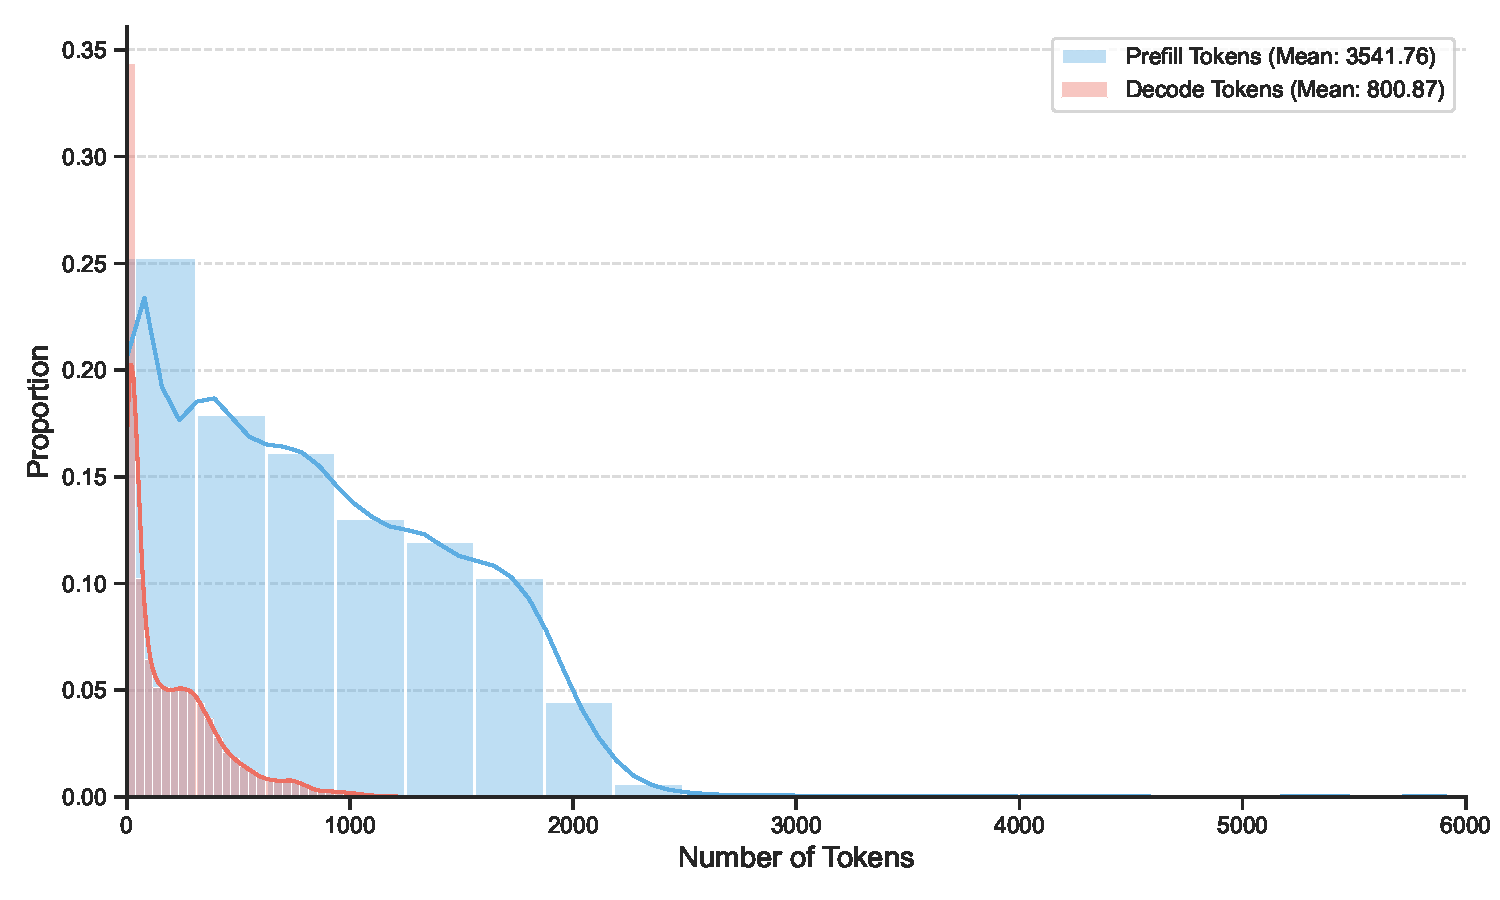
\includegraphics[width=\textwidth]{figures/5.2.a.pdf}
    \caption{ShareGPT数据集Token分布}
    \label{fig:top-left}
  \end{subfigure}
  \hfill
  \begin{subfigure}[b]{0.45\textwidth}
    \centering
    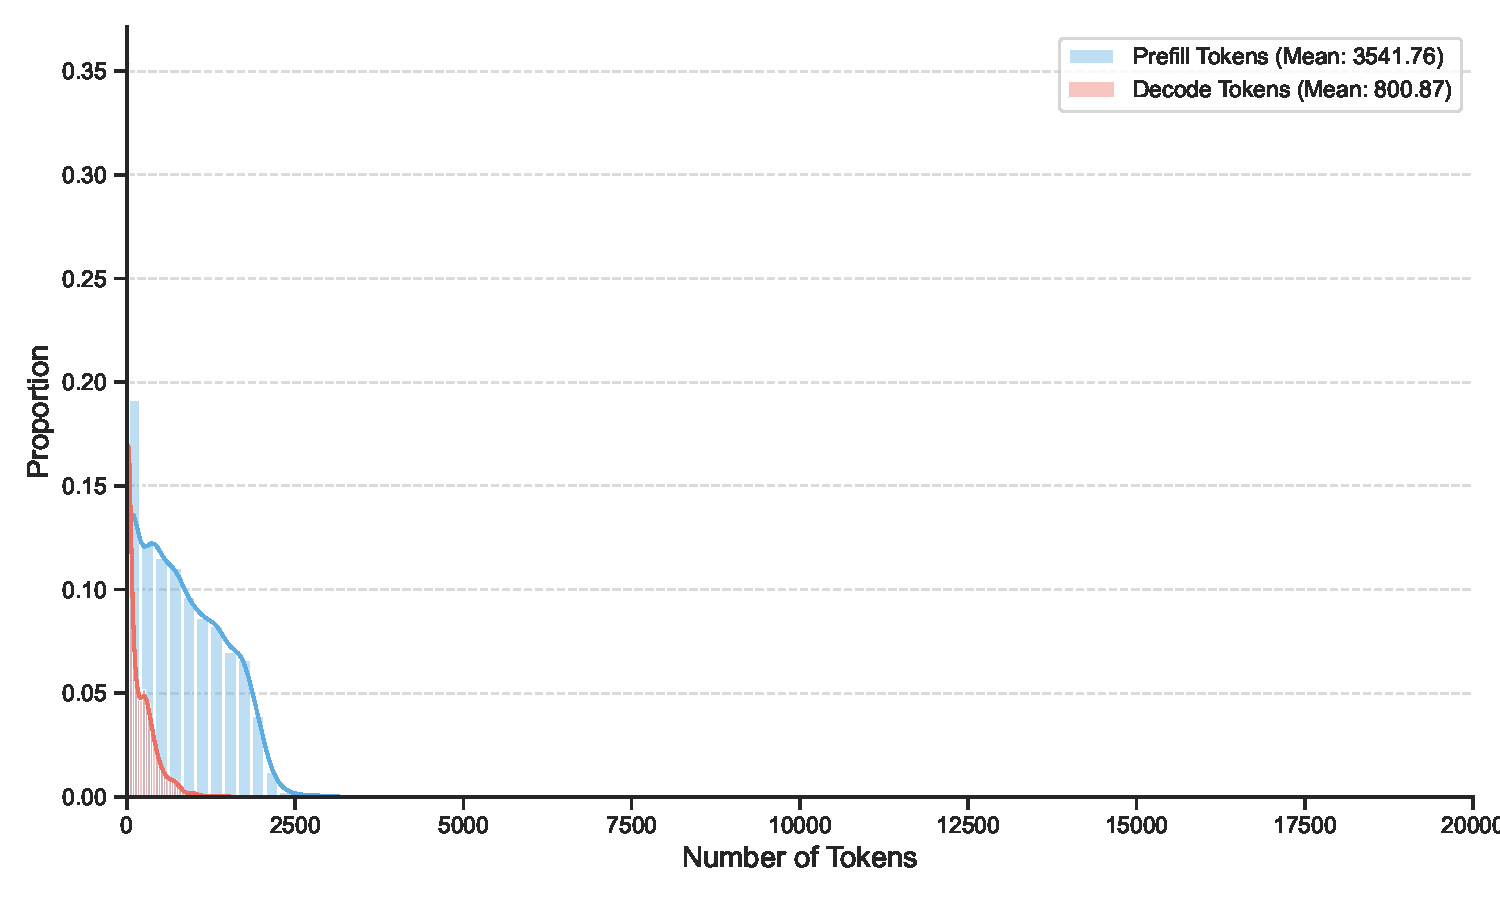
\includegraphics[width=\textwidth]{figures/5.2.b.pdf}
    \caption{Wikidata数据集Token分布}
    \label{fig:top-right}
  \end{subfigure}

  \vspace{1em}

  % --- 第二排 ---
  \begin{subfigure}[b]{0.45\textwidth}
    \centering
    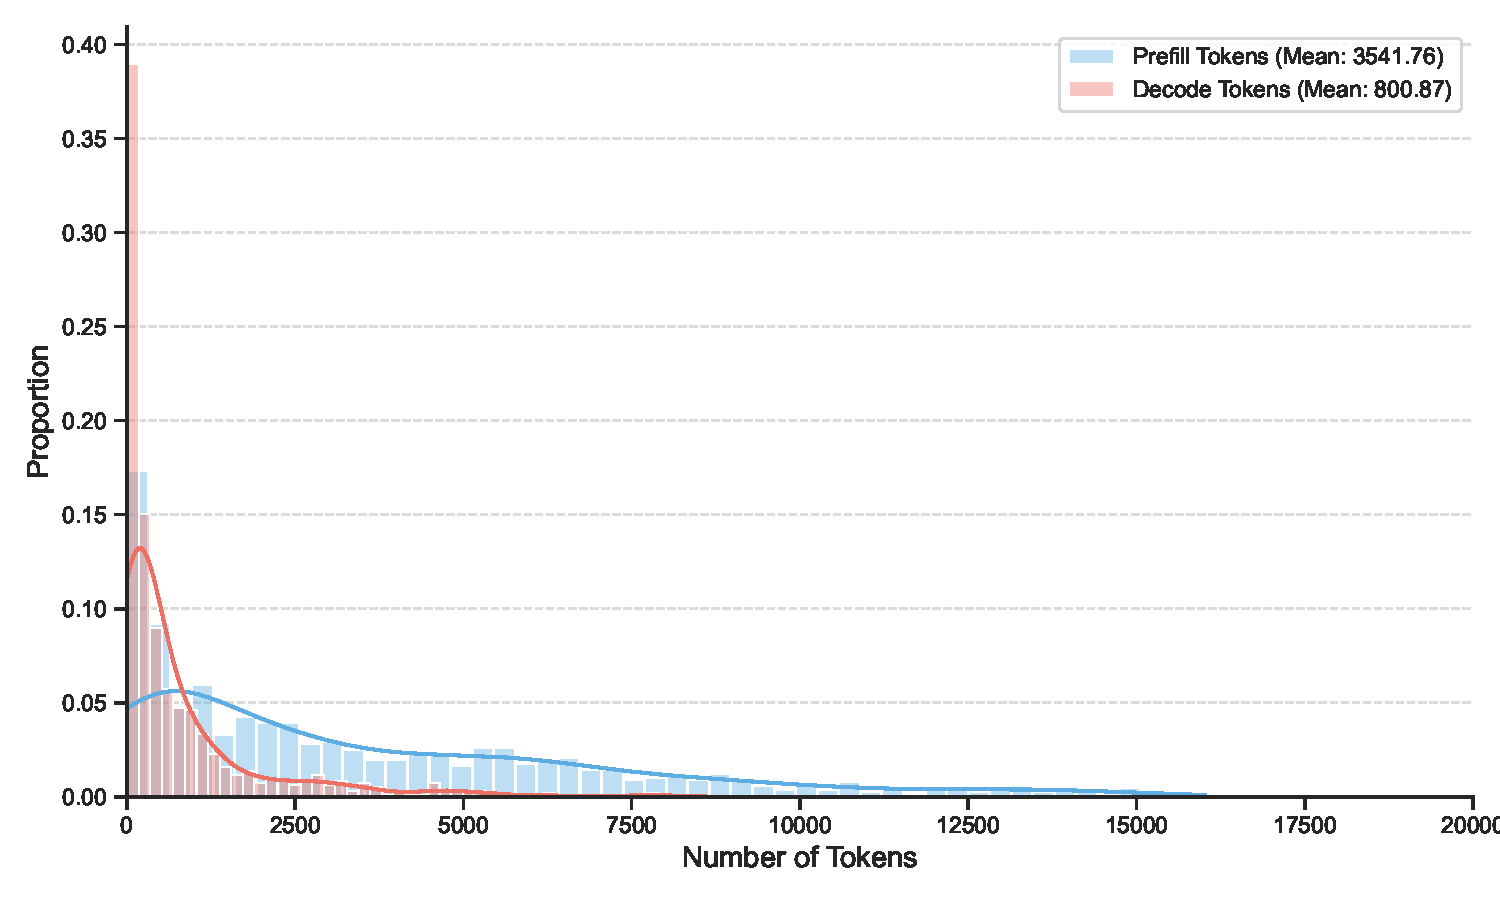
\includegraphics[width=\textwidth]{figures/5.2.c.pdf}
    \caption{CodeAgent数据集Token分布}
    \label{fig:bottom-left}
  \end{subfigure}
  \hfill
  \begin{subfigure}[b]{0.45\textwidth}
    \centering
    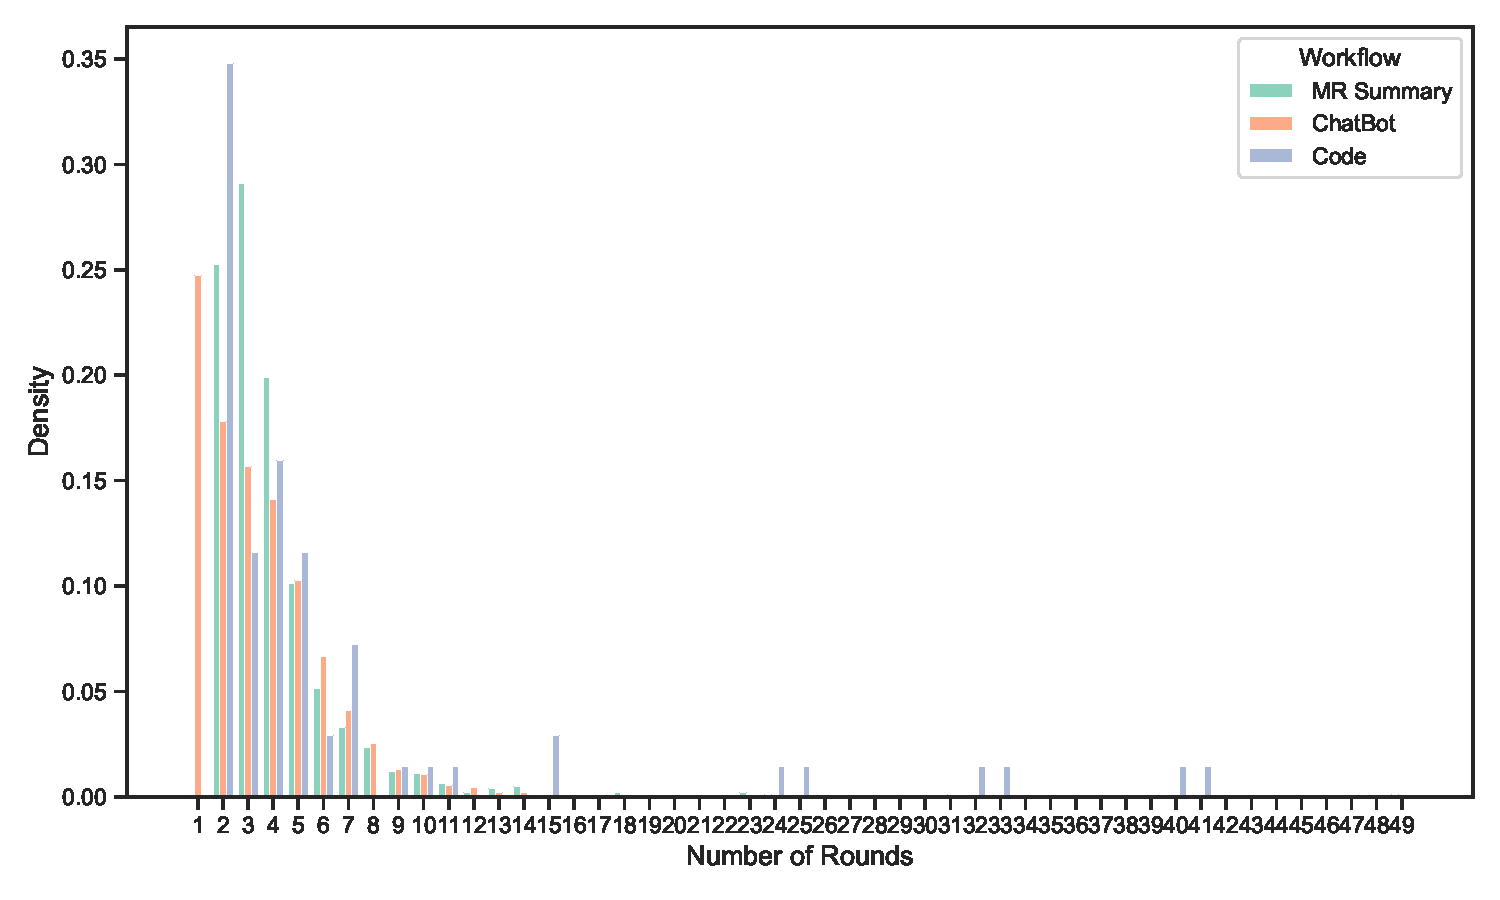
\includegraphics[width=\textwidth]{figures/5.2.d.pdf}
    \caption{不同工作流的请求数分布}
    \label{fig:bottom-right}
  \end{subfigure}

  \caption{不同Agent工作流的特征分布}
  \label{fig:four-images-total}
\end{figure}

本文的实验评估分为两步：首先分别测试三种单一的工作流负载，随后测试由这三种工作流按预设比例混合而成的混合负载。
为模拟真实的 LLM 推理服务轨迹，实验中的工作流到达时间均服从泊松分布。
在默认情况下，所有评估均基于 Llama3-8B 模型进行。


\subsection{对比方法与评估指标}

为验证所提方法的有效性，本文将其与以下基线方法进行对比：

\begin{itemize}
  \item \textbf{Round-Robin：}
        轮询策略（Round-Robin）默认采用先到先服务（FCFS）排队策略，并以轮询方式将请求均匀分发至各LLM实例。
        该方法不利用任何Agent工作流信息，是最基础的全局调度策略。

  \item \textbf{Parrot：}
        Parrot 是一套面向 LLM 应用的端到端服务系统。其核心通过语义变量抽象，
        使底层服务能够感知请求间的 DAG 依赖与提示词结构。
        在调度层面，Parrot 基于应用级性能目标对相似请求进行聚合；在分发层面，
        其采用会话亲和性机制，将关联请求定向路由至同一实例，以最大化 KV Cache 的前缀复用。
        作为对比算法，本文在仿真环境中仅复现了其核心的排队与分发策略，未包含其底层的工程级实现与优化。

  \item \textbf{Ayo：}
        Ayo是一个面向LLM应用的细粒度编排框架。
        其核心是将工作流转化为任务级数据流图，并辅以依赖剪枝与预填充拆分等图优化技术。在排队调度上，Ayo 
        依据拓扑结构优先处理处于工作流后期的请求；在实例分发上，
        则采用基础的轮询路由策略。同 Parrot 类似，
        本文的仿真对比仅严格复现了 Ayo 的拓扑排队与轮询分发机制，未包含其底层的图优化实现。
\end{itemize}
\noindent 为了全面评估并对比不同策略的性能，本文采用了以下核心指标：

\begin{itemize}
  \item \textbf{工作流平均端到端时延（Mean E2E Latency）}：
        从系统接收到Agent工作流的第一个请求到返回最终结果的平均端到端延迟，
        用于衡量系统在当前负载状态下的整体服务效率。

  \item \textbf{工作流P95端到端时延（P95 E2E Latency）}：
        指Agent工作流端到端延迟的第95百分位数，
        用于评估系统在高并发或极端负载下对长尾时延的控制能力及服务质量（QoS）保障水平。

  \item \textbf{P50首字时延（P50 TTFT）}：
        指请求被提交至LLM引擎到输出第一个Token的时延中位数，
        主要衡量请求在预填充阶段的排队等待耗时与上下文计算效率。

  \item \textbf{P50每Token输出时延（P50 TPOT）}：
        指在解码阶段中生成单个Token的时延的中位数，
        侧重反映 LLM 实例在自回归生成过程中的批处理效率。
\end{itemize}

\subsection{主要实验结果}

\begin{figure}[htbp]
  \centering
  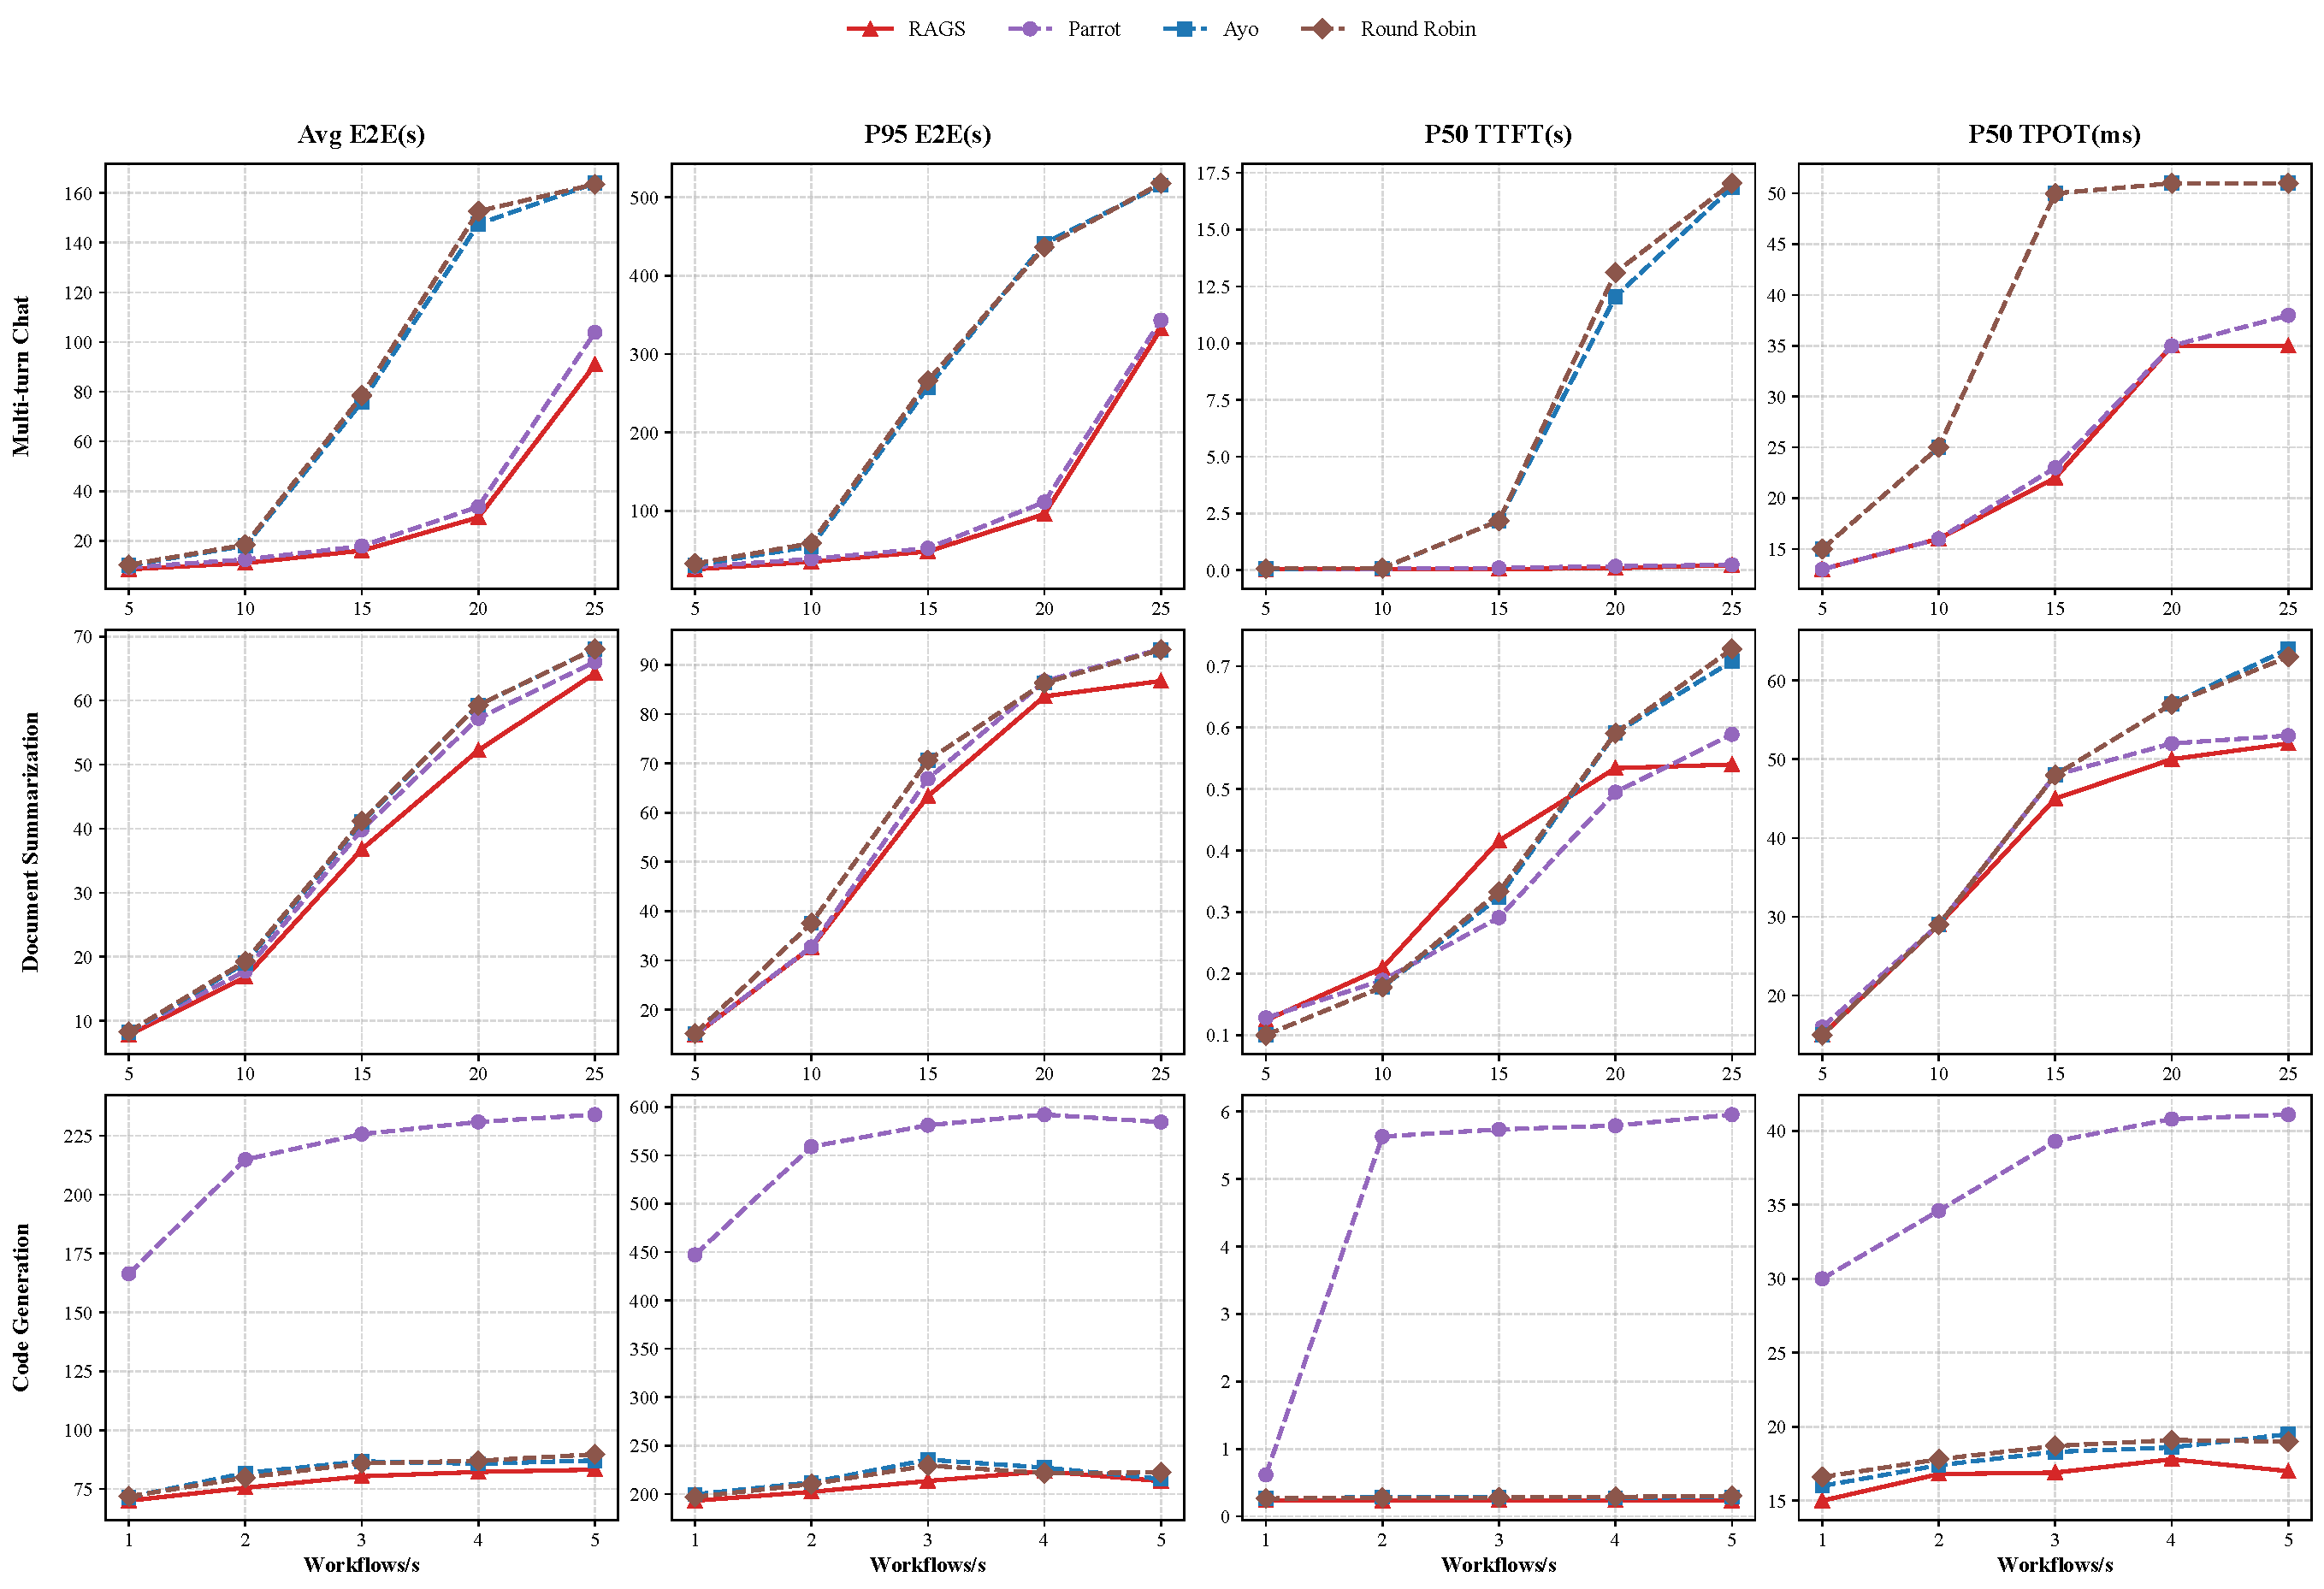
\includegraphics[width=\textwidth]{figures/5.3.pdf}
  \caption{不同请求率下的端到端性能对比}
  \label{fig:exp-e2e-latency}
\end{figure}

图~\ref{fig:exp-e2e-latency} 详细展示了在三种单一工作流负载下，各方法在不同请求到达率时的端到端性能。

多轮对话（ChatBot）场景旨在验证系统处理串行工作流的有效性。如图~\ref{fig:exp-e2e-latency}（第一行）所示，在并发量达 20 工作流/s 时，
RAGS 的平均端到端时延较 Round-Robin 和 Ayo 实现了最高 5.2 倍加速。在首字时延上，Round-Robin 的 P50 
指标随并发激增至 17 s，而 RAGS 凭借 RL 分发策略对集群负载的动态均衡与 DynA 对关键请求排队等待的压缩，将其稳定在 1 s 以内。值得注意的是，
该场景下 RAGS 较 Parrot 的加速比仅约 1.1 倍。其原因在于，ChatBot 拓扑较为固定且 KV 缓存共享模式呈现高度规律性，Parrot 
的静态前缀感知路由已能充分利用KV缓存。因此，在此类负载均匀的静态场景中，动态路由所带来的额外性能增益空间较为有限。

Map-Reduce 文档总结工作流同样具有高度规律性的固定两级拓扑（Map 并行与 Reduce 聚合），
因此，RAGS 相对各对比算法的综合增益亦较为有限。
如图~\ref{fig:exp-e2e-latency}（第二行）所示，当请求到达率为 20 工作流/s 时，
RAGS 的平均端到端时延相比 Round-Robin 仅降低约 6\%。
值得注意的是，由于工作流仅含两级拓扑，Ayo 基于拓扑排序的优先级策略难以区分海量同级 Map 节点，实质退化为轮询策略，
因此未获得明显增益。相比之下，DynA 通过估算工作流进度，
优先调度即将触发 Reduce 聚合的关键请求，一定程度上缓解了节点间的同步阻塞。

代码生成（CodeAgent）工作流引入了自主反馈优化机制，该场景旨在评估调度系统应对高度动态拓扑的能力。
如图~\ref{fig:exp-e2e-latency}（第三行）所示，Parrot 在此场景下引发了严重的队列拥塞，其平均端到端延迟高达 240 s，
P95 尾延迟达 600 s，分别约为 RAGS 的 3$\sim$4 倍。
其根本原因在于：代码修复的反馈循环导致各会话计算负载高度动态，
静态的会话亲和性策略极易引发全局负载失衡，部分复杂会话耗尽实例资源后，其他被亲和性绑定的请求遭遇严重队头阻塞。
得益于 RL 分发策略对动态负载的全局均衡与 DynA 对高优先级请求的抢先调度的协同作用，
RAGS 在大部分负载下将平均延迟稳定在 $70 \sim 85$ s；
在 P95 尾延迟方面，即使在 5 工作流/s 的并发压力下仍维持在 200 s 左右，优于 Ayo 与 Round-Robin。

TTFT 指标进一步揭示了各策略在高度动态负载下的队列拥塞程度差异。
随着并发请求率提升，Parrot 的 P50 TTFT 急剧恶化，在 5 工作流/s 时激增至约 6 s。
相比之下，RAGS 通过 RL 分发策略对显存利用率与集群负载的动态感知，以及 DynA 排队算法对关键请求的
优先处理，在 KV Cache 复用率与集群负载均衡之间实现了权衡。
因此，在同等高负载场景下，RAGS 仍能将 P50 TTFT 稳定控制在 0.5 s 以内，
表明排队与分发两级协同设计能够有效抑制动态工作流中的 TTFT 突增问题。

\textbf{混合负载下的性能评估。}
真实的生产环境往往伴随着高度异构的混合工作负载。为全面评估系统在复杂场景下的路由性能，
本实验构建了一个总规模为 500 个工作流请求的混合负载数据集，并按不同流量配比 $\left(x, y, z\right)$ 对上述三种典型工作流进行了混合
（其中 $x$、$y$、$z$ 分别代表这三种类型的 Agent 工作流在混合负载数据集中所占的比例）。其中工作流到达率
设置为 5 工作流/s。
图~\ref{fig:exp-e2e-latency-mix} 展示了不同策略在四组代表性混合配比下的平均端到端时延表现。
结果表明，本章提出的 RAGS 在各类混合场景中均展现出优异的泛化能力，并始终保持最低的时延水平。

\begin{figure}[htbp]
  \centering
  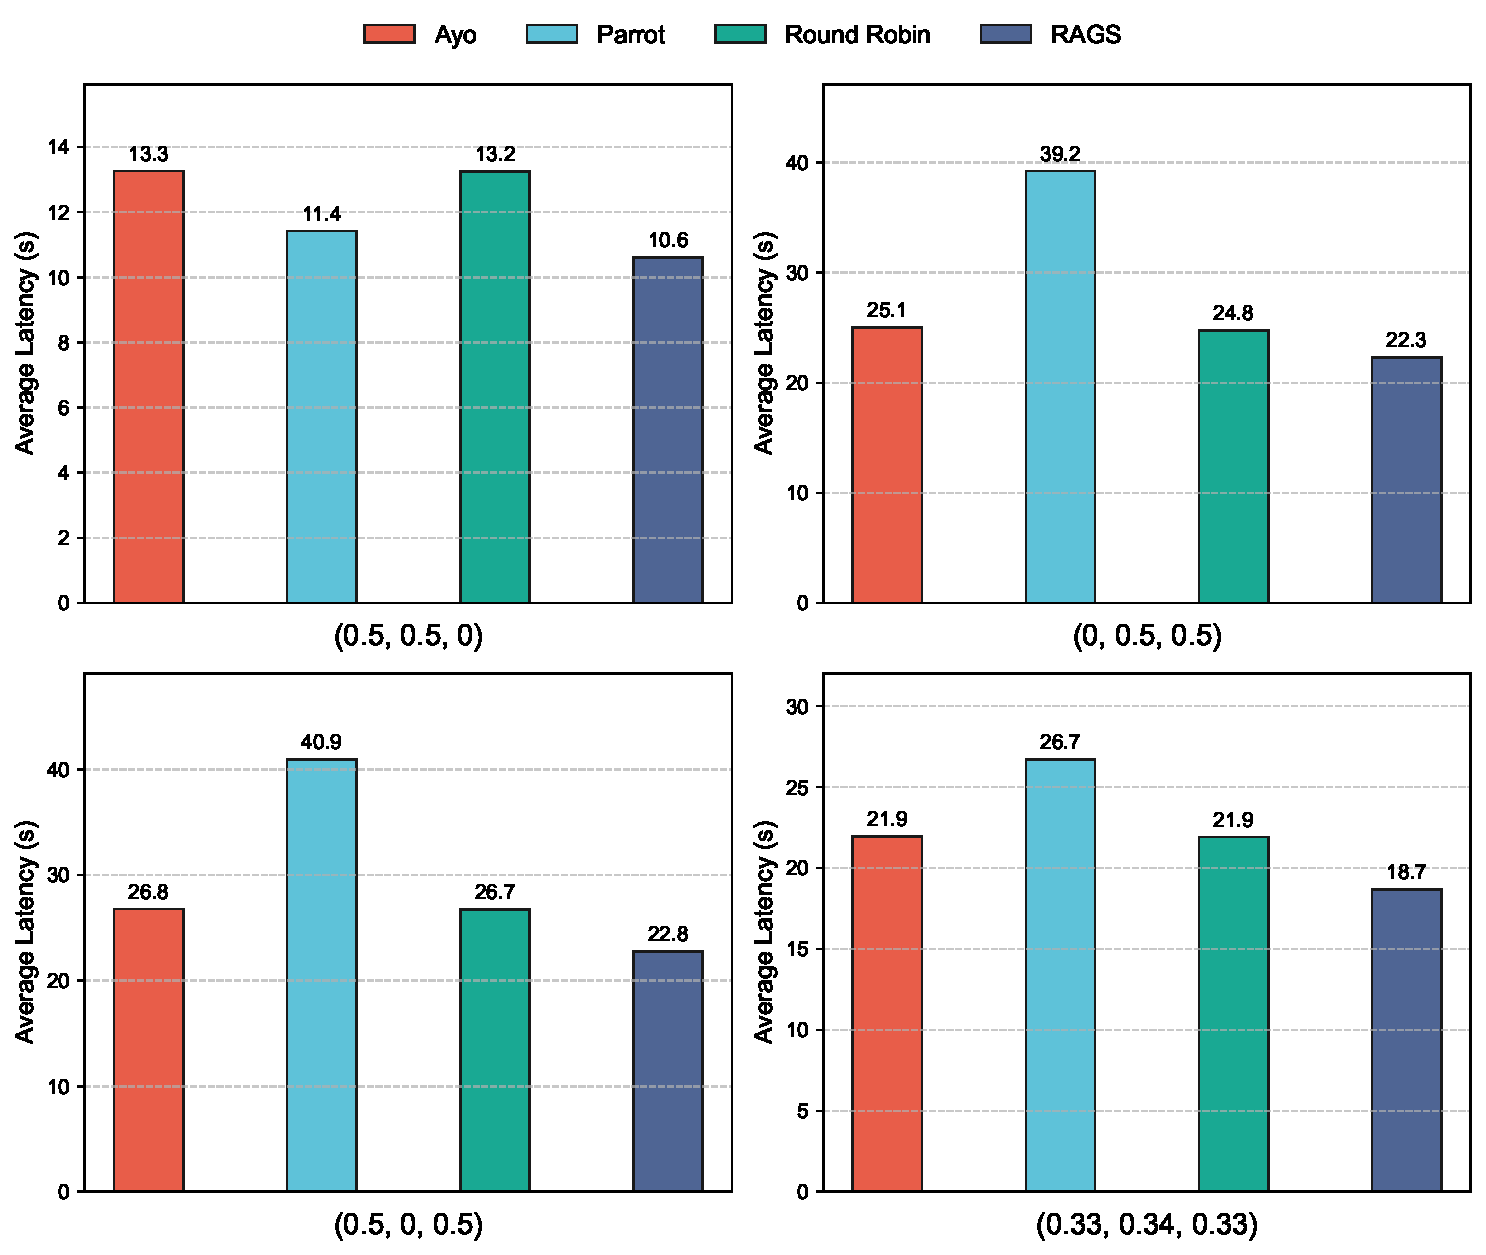
\includegraphics[width=\textwidth]{figures/5.4.pdf}
  \caption{混合负载下的端到端性能对比}
  \label{fig:exp-e2e-latency-mix}
\end{figure}

具体而言，当混合负载不包含代码生成任务（如配比 $\left(0.5, 0.5, 0\right)$）时，多数对比算法的时延集中在 $11\sim14\text{ s}$。
其中，Parrot 凭借会话亲和性带来的缓存复用取得了 $11.4\text{ s}$ 的次优表现，而 RAGS 以 $10.6\text{ s}$ 展现出最优的性能。
然而，一旦引入包含复杂反馈循环的代码生成任务（如配比 $\left(0, 0.5, 0.5\right)$ 与 $\left(0.5, 0, 0.5\right)$），Parrot 的时延急剧恶化至 $40\text{ s}$ 左右，
凸显了静态绑定策略在高计算密度下极易引发局部负载失衡的缺陷。同时，Ayo 与 Round-Robin 均展现出相似的性能退化，
表明仅依赖拓扑深度的静态排序难以应对异构并发流量。相比之下，RAGS 不仅在均衡混合场景 $\left(0.33, 0.34, 0.33\right)$ 中实现了 $18.7\text{ s}$ 
的平均时延（较 Ayo 降低 $14.5\%$，较 Parrot 降低 $28.6\%$），且在任意含代码生成的高压场景下，
均能将其端到端时延平稳控制在 $22.8\text{ s}$ 以内。

综上所述，RAGS 架构在处理具有时序依赖与高并发特征的复杂工作流时，展现出了较好的泛化能力与鲁棒性。这种端到端性能的提升，
根本上源于排队与分发策略的深度协同：在排队层，DynA 算法摆脱了对底层工作流图先验信息的依赖，
仅凭轻量级历史分布即可实现关键分支的自适应优先调度，在高负载场景下有效缓解了长尾延迟与请求饥饿；在分发层，RL 调度器实时整合实例负载特征进行路由，
成功突破了传统粗粒度亲和性策略导致的局部计算瓶颈。
实验结果充分证明了该双层全局路由架构在应对高度不确定性负载时的显著优势。



\subsection{对比实验}

为了探索不同超参数对RAGS性能的影响，本文首先对状态空间表示中的桶宽度$bin\_width$进行了对比实验。

\begin{figure}[htbp]
  \centering
  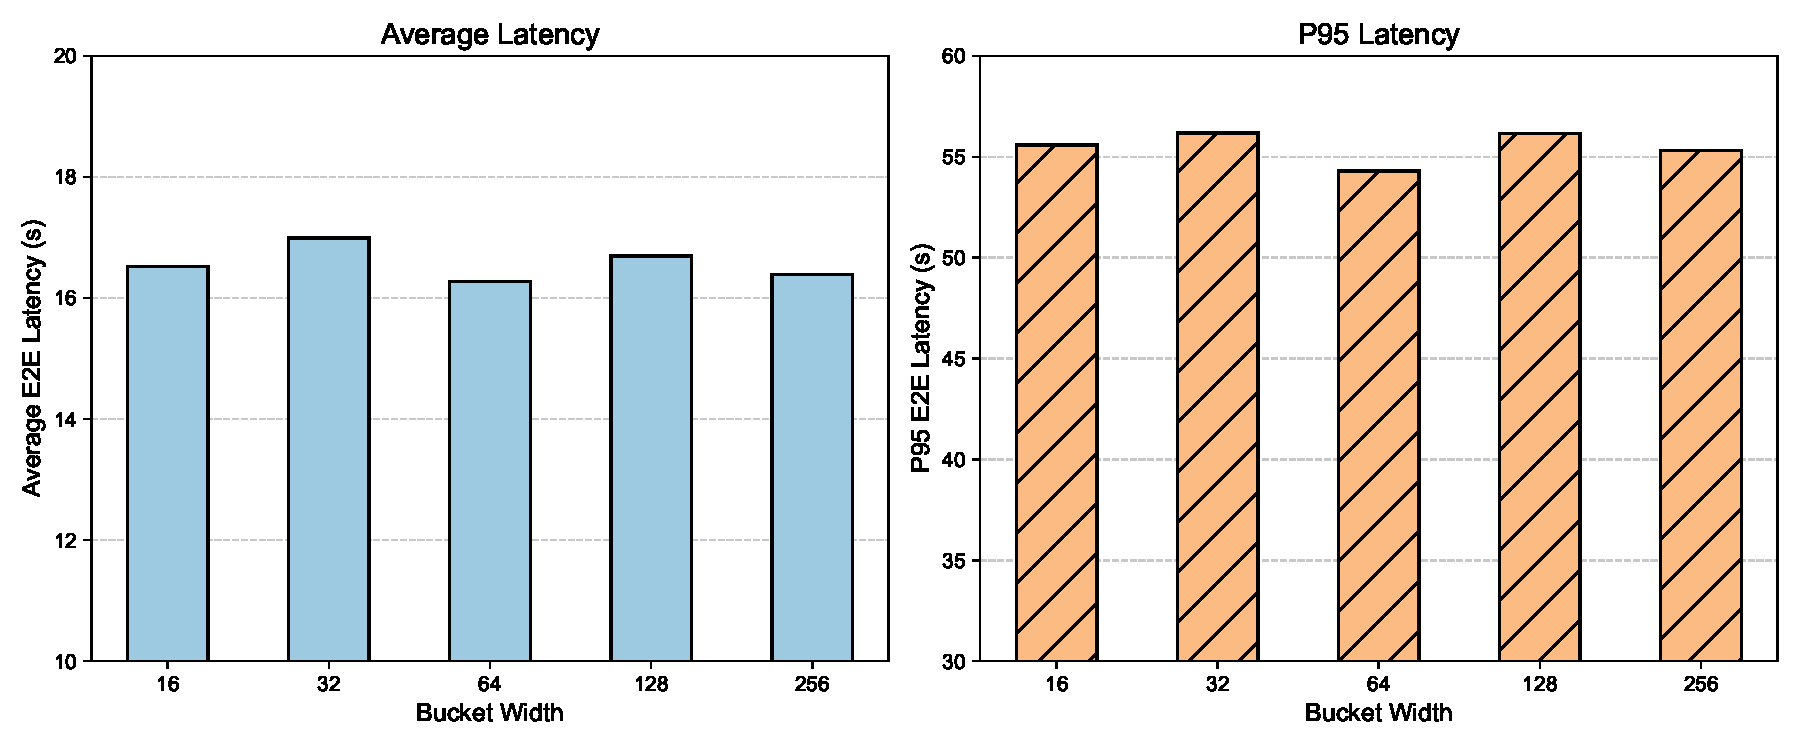
\includegraphics[width=\textwidth]{figures/5.5.pdf}
  \caption{不同桶宽度下的端到端性能对比}
  \label{fig:ablation-1}
\end{figure}

图~\ref{fig:ablation-1} 展示了桶宽度对系统端到端平均延迟的影响。实验结果表明，桶宽度的设定对模型性能具有显著影响：
若桶宽度过小，细粒度的状态空间表征会导致特征稀疏，增加强化学习模型的收敛难度；反之，若桶宽度过大，
粗粒度的状态划分会掩盖 LLM 实例间的负载差异，进而影响分发决策的精准性。
当桶宽度配置为64时，系统能够较好地平衡环境状态的表征精度与智能体的学习效率，实现最优的端到端性能。
因此，本文默认选用64作为桶宽度参数。

\subsection{消融实验}

此外，为评估排队策略与分发策略对系统性能的具体贡献，本文设计了针对核心调度组件的消融实验。
具体而言，本文采用混合工作负载（Chatbot : Summarization : Coding = 0.33 : 0.34 : 0.33），
对比了以下三种配置在不同请求到达率下的平均端到端延迟表现：
（1）\textbf{RAGS}：本章提出的完整方法，即DynA排队策略结合基于强化学习的分发策略；
（2）\textbf{RAGS w/o DynA}：移除DynA排队策略，退化为FCFS排队，仅保留强化学习分发策略；
（3）\textbf{RAGS w/o RL}：移除强化学习分发策略，退化为轮询策略，仅保留DynA排队策略。
图~\ref{fig:ablation-2} 详细展示了上述三种配置在不同请求到达率下的平均端到端延迟表现。

\begin{figure}[htbp]
  \centering
  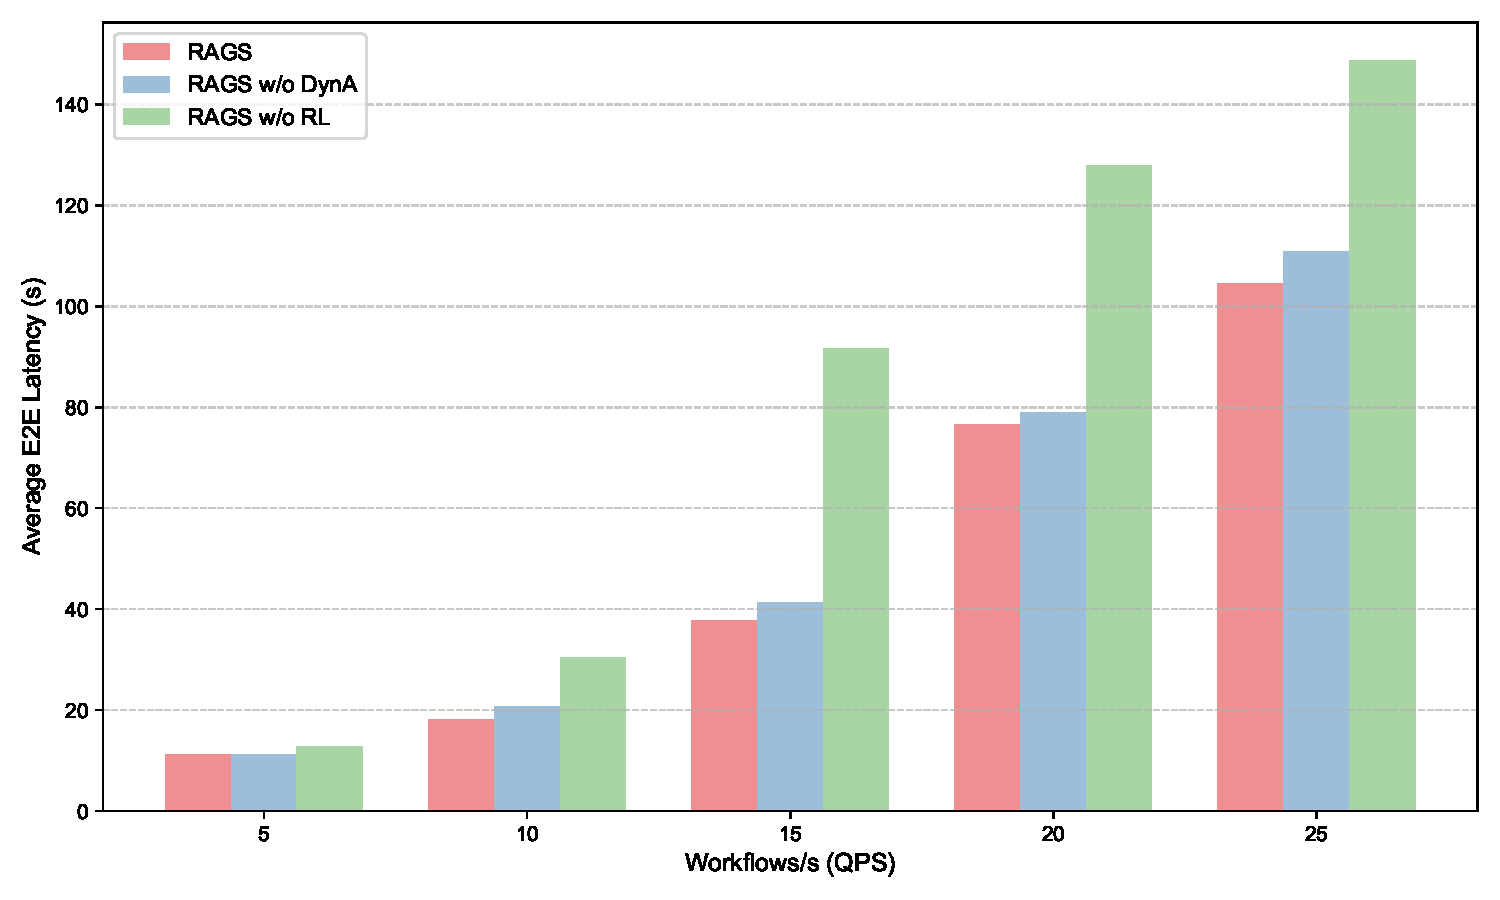
\includegraphics[width=0.8\textwidth]{figures/5.6.pdf}
  \caption{消融实验结果}
  \label{fig:ablation-2}
\end{figure}

实验结果表明，在低请求到达率下，三种配置的平均端到端延迟差异有限，
RAGS与RAGS w/o DynA分别为11.206 s和11.205 s，RAGS w/o RL为12.867 s，略高于前两者。
随着请求到达率的提升，三者之间的性能差距逐渐增大。
在最高请求到达率下，完整的RAGS实现了104.557 s的平均端到端延迟；
移除DynA排队策略的RAGS w/o DynA延迟上升至110.804 s；
移除RL分发策略的RAGS w/o RL则进一步劣化至148.758 s。

上述结果表明：
首先，RL分发策略对系统整体性能的贡献最为显著。RAGS w/o RL在高负载下的平均端到端延迟较完整方法增加了约42.27\%，
表明基于强化学习的分发策略的收益随系统负载升高而显著增大。
其次，DynA排队策略的贡献同样不可忽视。
在中等请求到达率下，RAGS w/o DynA的延迟较完整方法高出约14.8\%（20.782 s vs. 18.104 s），
表明DynA通过工作流进度感知的优先级排序有效缓解了队头阻塞，降低了关键路径请求的排队等待时间。
最后，两个调度组件之间存在协同增效关系：
DynA的优先级排序确保关键请求优先进入分发阶段，使RL智能体的负载均衡决策能够及时作用于最紧迫的请求；
RL的全局负载均衡则避免了关键请求在LLM引擎中的二次排队，从而在端到端层面保障了 DynA 优先级排序所预期的时延优化收益。

\subsection{异构场景对比实验}\label{subsec:chap4-heterogeneous}

\begin{figure}[htbp]
  \centering
  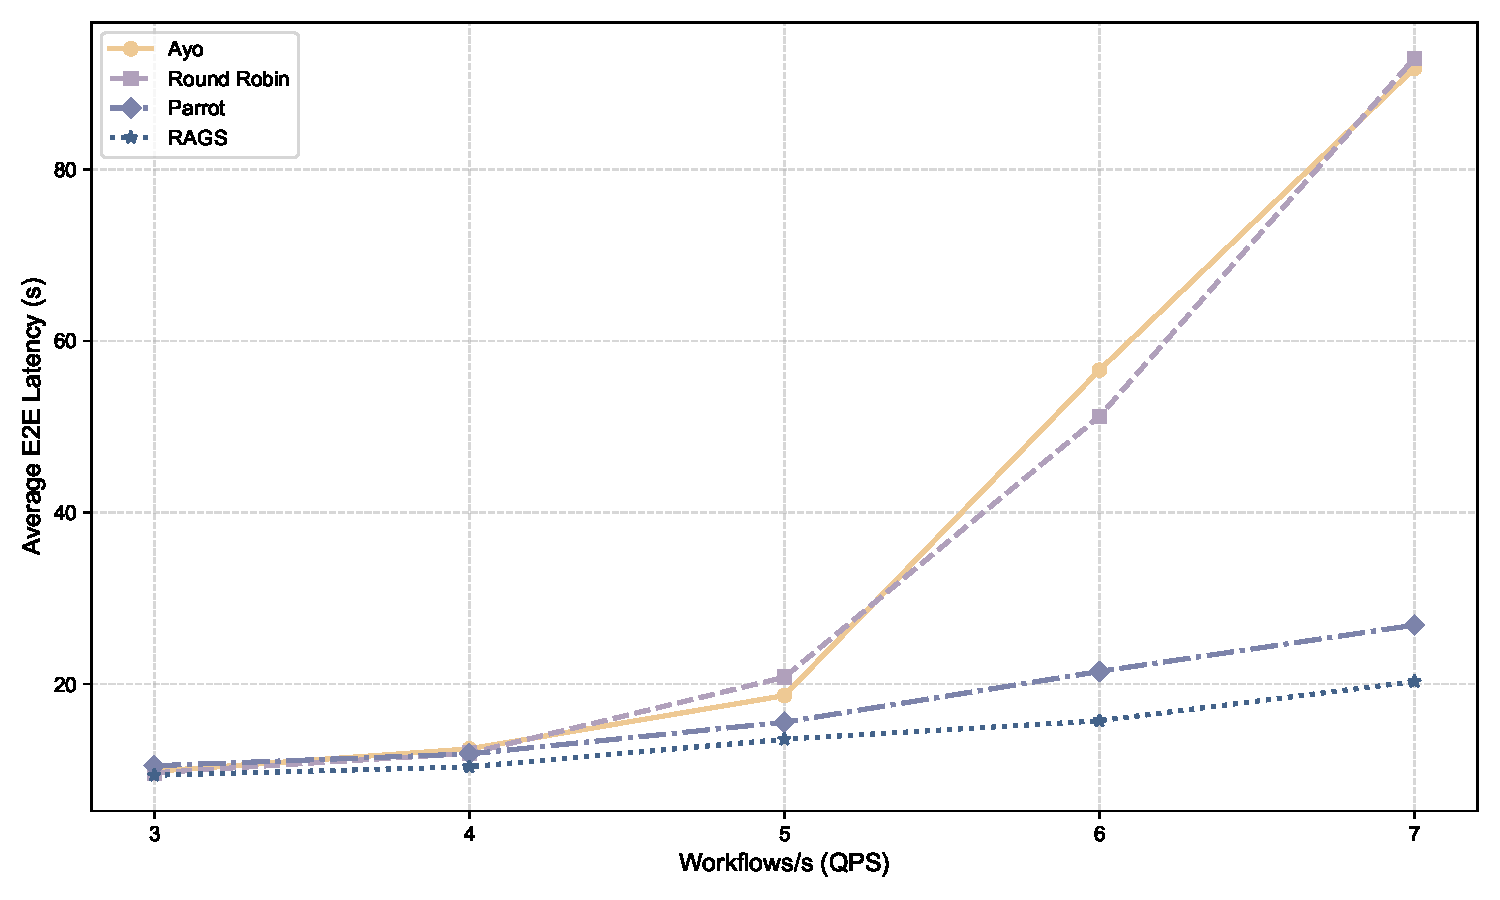
\includegraphics[width=0.8\textwidth]{figures/5.7.pdf}
  \caption{异构场景对比实验结果}
  \label{fig:heterogeneous-comparison}
\end{figure}

为验证RAGS在异构GPU集群中的调度能力，本文在由2块NVIDIA A100与2块NVIDIA H100组成的4卡推理集群上开展对比实验。
鉴于 H100 架构下 Meta-Llama-3-8B 模型的性能基准数据尚不完备，各实例均统一采用 meta-llama/Llama-2-7b-hf 模型进行部署。
此外，考虑到A100与H100在计算吞吐量和显存带宽上存在显著差异，异构集群的调度器需要在请求分发时感知实例的硬件异质性，
同时避免因负载分配不均导致的资源浪费。

如图~\ref{fig:heterogeneous-comparison} 所示，当请求到达率从3 提升至7 workflow/s时，
各方法的平均端到端延迟均呈上升趋势，但上升幅度存在显著差异。
Round-Robin 策略因未考虑 GPU 的异构性进行均匀分发，导致算力较弱的 A100 实例沦为系统性能瓶颈，
高并发下的队列积压使其端到端延迟飙升至 80 s 以上。
同时，尽管 Parrot 利用了会话亲和性提升 KV 缓存复用率，
但其静态绑定机制同样缺乏对底层算力差异的感知。
当高计算密度的请求被固定分配至算力较弱的 A100 实例时，
极易引发严重的局部过载。

相比之下，RAGS在不同负载强度下均维持了最低的平均端到端延迟。
这一优势源于强化学习状态空间对 GPU 类型与实例负载的联合编码：
调度策略能够隐式感知实例间的算力差异，从而在分发决策中自适应地兼顾硬件性能与全局负载均衡，
避免了静态绑定策略对异构硬件的盲目分配。
实验表明，在7 workflow/s的峰值负载下，RAGS较Round-Robin与Parrot将平均端到端延迟
降低了约30\%至40\%，验证了该方法在异构推理集群中的有效性与泛化能力。

\section{本章小结}\label{sec:chap4-summary}

针对多租户LLM Agent服务场景中传统调度策略无法感知工作流依赖关系与异构请求特征、
从而导致队头阻塞和负载不均等问题，
本文提出了全局调度算法 RAGS。在排队策略上，本文提出了动态感知排队算法 DynA，
通过在线维护各Agent类型的完成轮次分布并基于条件近完成概率构建综合优先级分数，
在无需预知工作流拓扑结构的前提下实现了Agent间与Agent内两个层次的自适应优先级排序。
针对分发策略，本章将请求路由过程转化为马尔可夫决策过程，进而利用强化学习算法求解最优分发策略。
在模型构建上，本文采用了基于 Transformer 的策略网络，
并设计了兼顾延迟、排队等待与负载均衡的复合奖励函数；
为保障系统在动态环境下的自适应能力，进一步采用离线预训练与在线微调相结合的两阶段范式，从而实现了智能体的高效迭代。
实验结果表明，RAGS在多种典型Agent工作流及混合负载场景下均优于现有方法，
消融实验与异构集群实验进一步验证了两个调度组件的协同效应与泛化能力。
需要指出的是，本章实验均在Vidur仿真平台上开展，主要目的是验证算法的可行性与有效性；
未来工作将考虑在真实LLM推理集群上进行实机部署实验，以进一步评估系统在生产环境中的实际性能。

\cleardoublepage
